\chapter{\glspl{manet} and Trust}
\label{ch:trust_background}
\lhead{Chapter \thechapter. \emph{\glspl{manet} and Trust}}

\section{\acrlong{manet} Topologies \& Routing}\label{sec:manet_topologies}

\glspl{manet} are wireless networks consisting of mobile devices acting simultaneously as sensor/processing/effector nodes and routing nodes, acting without a classical \gls{wlan} structured network architecture. 
Given constraints on propagation in such wireless networks, it is impractical for nodes to be ``fully connected'' to the rest of the network, and is instead constructed from single-hop ``node-pair'' links, through and across which data is routed to more distant parts of the network.
This link-wise approach coupled with inherant Node mobility results in a potentially highly dynamic topology, where the instantaneous graph of node-pair connectivity can change dramatically in short intervals, and it may take considerable time for the network to ``re-optimise'' for this new, possibly temporary, topology. 

In order to understand and clarify the challenges to generic \gls{manet} applications, it is beneficial to explore some concepts from Graph Theory that apply to the discussion of \gls{manet} topologies. 


\begin{table} 
	\centering
	\begin{tabular}{cc}
		\toprule
		Graph Theory & Network Engineering\\
		\midrule
		Vertex & Node\\
		Edge & Link\\
		Undirected & Symmetric\\
		Directed & Asymmetric\\
		\bottomrule
	\end{tabular}
	\caption{Basic mapping between Graph and Network Theory nomenclatures}
\end{table}

\subsection{Network Density and Connectivity}

One fundamental compromise in the operation of wireless \glspl{manet} is the trade-off between the number of hops required between source and destination nodes and the effective bandwidth available to the network overall~\cite{Royer2001}.
This compromise is encapsulated in the relative density of a given network; that is, the number of nodes in a given node's one-hop locality, drawing direct links between wireless transmission strength / reception sensitivity, the environmental noise floor, environmental channel characteristics, the mobility of the nodes and the number of nodes deployed in a region.

From graph theory, the concept of ``Density'' is a $D_G=[0,1]$ bounded measure of how ``Complete'' or fully-connected a given graph $G$ consisting of the set of vertices $V$ and edges (links) $E$ is.
``Connectivity'' can be generalised as the routing-ability and the possible redundancy of that routing-ability across the graph, i.e.\ for a ``Connected'' graph, such that there is a sequence of edges (a path) that can be traversed to link all possible pairs of nodes, but if any of the nodes were removed, the graph becomes disconnected or separated, that graph has a connectivity of $1$.
If this is not possible, but it is possible to disconnect the graph by removing two vertices, the graph has connectivity 2, and so on.
A graph with a connectivity of $0$ indicates that that graph has separated (or disconnected) vertices.

The concepts of graph density and connectivity are demonstrated visually in \autoref{fig:manet_density}, constructed with a uniform vertex distribution and decomposed by removing subsequent ``longest edges'' from a fully connected (Complete) graph.

\todo{ADD: Need a ``Centralised/DeCentralised/Distributed'' graph series}

\tikzstyle{cblue}=[circle, draw, thin,fill=cyan!20, scale=0.8]

\begin{figure}

	\begin{subfigure}[t]{0.5\textwidth}
		\centering
		\begin{tikzpicture}[>=latex',scale=1]
		% Physical layer nodes
		\foreach \x/\place in {{1/(-2.5, 0.3)},{2/(-1.75, -0.55)},{3/(-1.2, 0.55)},{4/(-0.75, -0.7)},{5/(-0.25, 0)},{6/(0.25, 0.7)},{7/(0.75, -0.3)},{8/(1.5, 0)},{9/(2.5, 0.4)}}
			\node[cblue] (a\x) at \place {};
		\foreach \x/\y in {{1/2},{1/3},{1/4},{1/5},{1/6},{1/7},{1/8},{1/9},{2/3},{2/4},{2/5},{2/6},{2/7},{2/8},{2/9},{3/4},{3/5},{3/6},{3/7},{3/8},{3/9},{4/5},{4/6},{4/7},{4/8},{4/9},{5/6},{5/7},{5/8},{5/9},{6/7},{6/8},{6/9},{7/8},{7/9},{8/9}}
			% Physical layer links
			\path[thin] (a\x) edge (a\y);
		\end{tikzpicture}
		\caption{Fully connected (Complete) ($D=1.0, k=8.0$}
	\end{subfigure}
	\begin{subfigure}[t]{0.5\textwidth}
		\centering
		\begin{tikzpicture}[>=latex',scale=1]
		% Physical layer nodes
		\foreach \x/\place in {{1/(-2.5, 0.3)},{2/(-1.75, -0.55)},{3/(-1.2, 0.55)},{4/(-0.75, -0.7)},{5/(-0.25, 0)},{6/(0.25, 0.7)},{7/(0.75, -0.3)},{8/(1.5, 0)},{9/(2.5, 0.4)}}
			\node[cblue] (a\x) at \place {};
		\foreach \x/\y in {{1/2},{1/3},{1/4},{1/5},{2/3},{2/4},{2/5},{3/4},{3/5},{3/6},{3/7},{4/5},{4/6},{4/7},{5/6},{5/7},{5/8},{6/7},{6/8},{6/9},{7/8},{7/9},{8/9}}
			% Physical layer links
			\path[thin] (a\x) edge (a\y);
		\end{tikzpicture}
		\caption{($D=0.64,k=3$)}
	\end{subfigure}
	\begin{subfigure}[t]{0.5\textwidth}
		\centering
		\begin{tikzpicture}[>=latex',scale=1]
		% Physical layer nodes
		\foreach \x/\place in {{1/(-2.5, 0.3)},{2/(-1.75, -0.55)},{3/(-1.2, 0.55)},{4/(-0.75, -0.7)},{5/(-0.25, 0)},{6/(0.25, 0.7)},{7/(0.75, -0.3)},{8/(1.5, 0)},{9/(2.5, 0.4)}}
			\node[cblue] (a\x) at \place {};
		\foreach \x/\y in {{1/2},{1/3},{2/3},{2/4},{2/5},{3/4},{3/5},{3/6},{4/5},{4/6},{4/7},{5/6},{5/7},{5/8},{6/8},{6/7},{7/8},{8/9}}
			% Physical layer links
			\path[thin] (a\x) edge (a\y);
		\end{tikzpicture}
		\caption{($D=0.5,k=1$)}
	\end{subfigure}
	\begin{subfigure}[t]{0.5\textwidth}
		\centering
		\begin{tikzpicture}[>=latex',scale=1]
		% Physical layer nodes
		\foreach \x/\place in {{1/(-2.5, 0.3)},{2/(-1.75, -0.55)},{3/(-1.2, 0.55)},{4/(-0.75, -0.7)},{5/(-0.25, 0)},{6/(0.25, 0.7)},{7/(0.75, -0.3)},{8/(1.5, 0)},{9/(2.5, 0.4)}}
				 \node[cblue] (a\x) at \place {};
		\foreach \x/\y in {{1/2},{2/4},{3/5},{4/5},{5/6},{5/7},{7/8},{8/9}}
		% Physical layer links
		\path[thin] (a\x) edge (a\y);
		\end{tikzpicture}
		\caption{Minimally Connected ($D=0.22,k=1$)}
	\end{subfigure}
	\begin{subfigure}[t]{0.5\textwidth}
		\centering
		\begin{tikzpicture}[>=latex',scale=1]
		% Physical layer nodes
		\foreach \x/\place in {{1/(-2.5, 0.3)},{2/(-1.75, -0.55)},{3/(-1.2, 0.55)},{4/(-0.75, -0.7)},{5/(-0.25, 0)},{6/(0.25, 0.7)},{7/(0.75, -0.3)},{8/(1.5, 0)},{9/(2.5, 0.4)}}
				 \node[cblue] (a\x) at \place {};
		\foreach \x/\y in {{2/4},{3/5},{4/5},{5/6},{5/7},{7/8},{8/9}}
		% Physical layer links
		\path[thin] (a\x) edge (a\y);
		\end{tikzpicture}
		\caption{Disconnected ($D=0.19,k=0$)}
	\end{subfigure}
	\begin{subfigure}[t]{0.5\textwidth}
		\centering
		\begin{tikzpicture}[>=latex',scale=1]
		% Physical layer nodes
		\foreach \x/\place in {{1/(-2.5, 0.3)},{2/(-1.75, -0.55)},{3/(-1.2, 0.55)},{4/(-0.75, -0.7)},{5/(-0.25, 0)},{6/(0.25, 0.7)},{7/(0.75, -0.3)},{8/(1.5, 0)},{9/(2.5, 0.4)}}
		\node[cblue] (a\x) at \place {};
		\end{tikzpicture}
		\caption{An Empty Graph ($D=0,k=0$)}
	\end{subfigure}
	\caption{Network Density and Connectivity Examples}
	\label{fig:manet_density}
\end{figure}


\subsection{Node Density in \glspl{manet}}

In practical wireless network applications, network connectivity is a product of the physical distribution of nodes within an environment, and the propagation characteristics of the medium.

Taking the same physical configuration as in \autoref{fig:manet_density}, the structure, density and connectivity of the network with different assumed propagation ranges $r$ can be shown. 
\todo{ADD:Need some ``observations'' on the impacts of this routing constraint in manets in terms of \autoref{fig:manet_topo_states}\autoref{fig:manet_topo_mobility}}

\begin{figure}
	\begin{subfigure}[t]{0.5\textwidth}
		\centering
		\begin{tikzpicture}[>=latex',scale=1]
		% Physical layer nodes
		\foreach \x/\place in {{1/(-2.5, 0.3)},{2/(-1.75, -0.55)},{3/(-1.2, 0.55)},{4/(-0.75, -0.7)},{5/(-0.25, 0)},{6/(0.25, 0.7)},{7/(0.75, -0.3)},{8/(1.5, 0)},{9/(2.5, 0.4)}}
		\node[cblue] (a\x) at \place {};
		\foreach \x/\y in {{1/2},{1/3},{1/4},{1/5},{2/3},{2/4},{2/5},{2/6},{3/4},{3/5},{3/6},{3/7},{4/5},{4/6},{4/7},{4/8},{5/6},{5/7},{5/8},{6/7},{6/8},{6/9},{7/8},{7/9},{8/9}}
		% Physical layer links
		\path[thin] (a\x) edge (a\y);
		\draw [line width=0.1em] (1.5,-1) -- node[below,inner sep=0.1em, font=\footnotesize] {1 Unit} (2.5,-1);
		\end{tikzpicture}
		\caption{($r=2.5,D=0.69,k=3$)}
	\end{subfigure}
	\begin{subfigure}[t]{0.5\textwidth}
		\centering
		\begin{tikzpicture}[>=latex',scale=1]
		% Physical layer nodes
		\foreach \x/\place in {{1/(-2.5, 0.3)},{2/(-1.75, -0.55)},{3/(-1.2, 0.55)},{4/(-0.75, -0.7)},{5/(-0.25, 0)},{6/(0.25, 0.7)},{7/(0.75, -0.3)},{8/(1.5, 0)},{9/(2.5, 0.4)}}
		\node[cblue] (a\x) at \place {};
		\foreach \x/\y in {{1/2},{1/3},{2/3},{2/4},{2/5},{3/4},{3/5},{3/6},{4/5},{4/6},{4/7},{5/6},{5/7},{5/8},{6/8},{6/7},{7/8},{7/9},{8/9}}
		% Physical layer links
		\path[thin] (a\x) edge (a\y);
		\draw [line width=0.1em] (1.5,-1) -- node[below,inner sep=0.1em, font=\footnotesize] {1 Unit} (2.5,-1);
		\end{tikzpicture}
		\caption{($r=2,D=0.53,k=2$)}
	\end{subfigure}
	\begin{subfigure}[t]{0.5\textwidth}
		\centering
		\begin{tikzpicture}[>=latex',scale=1]
		% Physical layer nodes
		\foreach \x/\place in {{1/(-2.5, 0.3)},{2/(-1.75, -0.55)},{3/(-1.2, 0.55)},{4/(-0.75, -0.7)},{5/(-0.25, 0)},{6/(0.25, 0.7)},{7/(0.75, -0.3)},{8/(1.5, 0)},{9/(2.5, 0.4)}}
		\node[cblue] (a\x) at \place {};
		\foreach \x/\y in {{1/2},{1/3},{2/3},{2/4},{3/4},{3/5},{3/6},{4/5},{5/6},{5/7},{6/8},{6/7},{7/8},{8/9}}
		% Physical layer links
		\path[thin] (a\x) edge (a\y);
		\draw [line width=0.1em] (1.5,-1) -- node[below,inner sep=0.1em, font=\footnotesize] {1 Unit} (2.5,-1);
		\end{tikzpicture}
		\caption{($r=1.5,D=0.39,k=1$)}
	\end{subfigure}
	\begin{subfigure}[t]{0.5\textwidth}
		\centering
		\begin{tikzpicture}[>=latex',scale=1]
		% Physical layer nodes
		\foreach \x/\place in {{1/(-2.5, 0.3)},{2/(-1.75, -0.55)},{3/(-1.2, 0.55)},{4/(-0.75, -0.7)},{5/(-0.25, 0)},{6/(0.25, 0.7)},{7/(0.75, -0.3)},{8/(1.5, 0)},{9/(2.5, 0.4)}}
		\node[cblue] (a\x) at \place {};
		\foreach \x/\y in {{4/5},{5/6},{7/8}}
		% Physical layer links
		\path[thin] (a\x) edge (a\y);
		\draw [line width=0.1em] (1.5,-1) -- node[below,inner sep=0.1em, font=\footnotesize] {1 Unit} (2.5,-1);
		\end{tikzpicture}
		\caption{($r=1,D=0.08,k=0$)}
	\end{subfigure}
	\caption{Examples of states of \gls{manet} topologies}
	\label{fig:manet_topo_states}
\end{figure}
\begin{figure}
	\begin{subfigure}[t]{0.5\textwidth}
	  	\centering
		\begin{tikzpicture}[>=latex',scale=1]
			 % Physical layer nodes
			 \foreach \x/\place in {{1/(-2.5, 0.3)},{2/(-1.75, -0.55)},{3/(-1.2, 0.55)},{4/(-0.75, -0.7)},{5/(-0.25, 0)},{6/(0.25, 0.7)},{7/(0.75, -0.3)},{8/(1.5, 0)},{9/(2.5, 0.4)}}
				 \node[cblue] (a\x) at \place {\x};
			 \foreach \x/\y in {{1/2},{1/3},{2/3},{2/4},{3/4},{3/5},{3/6},{4/5},{5/6},{5/7},{6/8},{6/7},{7/8},{8/9}}
			  % Physical layer links
				  \path[thin] (a\x) edge (a\y);
		\end{tikzpicture}
	  	\caption{Initial State}
	\end{subfigure}
	\begin{subfigure}[t]{0.5\textwidth}
		\centering
		\begin{tikzpicture}[>=latex',scale=1]
		% Physical layer nodes
		\foreach \x/\place in {{1/(-2.5, 0.3)},{2/(-1.75, -0.55)},{3/(-1.2, 0.55)},{4/(-0.75, -0.7)},{5/(-0.25, 0)},{6/(0.25, 0.7)},{7/(0.75, -0.3)},{8/(1.5, 0)},{9/(2.8, 0.8)}}
		\node[cblue] (a\x) at \place {\x};
		\foreach \x/\y in {{1/2},{1/3},{2/3},{2/4},{3/4},{3/5},{3/6},{4/5},{5/6},{5/7},{6/8},{6/7},{7/8}}
		% Physical layer links
		\path[thin] (a\x) edge (a\y);
		
		\path[dashed] (a8) edge (a9);
		
		\draw [->] (a9) -- (3.2, 1.3);			
		\end{tikzpicture}
		\caption{Node $9$ moves out of range and loses connectivity}
		\end{subfigure}
		\begin{subfigure}[t]{0.5\textwidth}
			\centering
			\begin{tikzpicture}[>=latex',scale=1]
			% Physical layer nodes
			\foreach \x/\place in {{1/(-2.5, 0.3)},{2/(-1.75, -0.55)},{3/(-1.2, 0.55)},{4/(-0.75, -0.7)},{5/(-0.25, 0)},{6/(0.25, 0.7)},{7/(0.75, -0.3)},{8/(1.5, 0)},{9/(-1, -1.4)}}
			\node[cblue] (a\x) at \place {\x};
			\foreach \x/\y in {{1/2},{1/3},{2/3},{2/4},{2/9},{3/4},{3/5},{3/6},{4/9},{4/5},{5/6},{5/7},{6/8},{6/7},{7/8}}
				% Physical layer links
				\path[thin] (a\x) edge (a\y);
			\end{tikzpicture}
			\caption{Node 9 rejoins the network}
		\end{subfigure}
		\caption{Example of node mobility of \gls{manet} topologies}
		\label{fig:manet_topo_mobility}
\end{figure}


\section{Routing in \acrlongpl{manet}}\label{sec:manet_routing}

Given the decentralised nature of \gls{manet} operations, routing protocols have been an active area of research since their inception~\cite{Jubin1987}.
This research is classified according to the strategies used for discovering, monitoring and updating routes within the network, and are usually grouped into three classes; proactive (or Table Driven), reactive (or On Demand) and hybrid protocols.
A summary of the generalised characteristics of these classes is shown in \autoref{tab:routing_categories}.
Additional, these classes can be further rearranged, combined or augmented based on assumptions made about the structure of the baseline topology, i.e. flat, hierarchical or geographic) or by assumed constraints of the available resources of the nodes within the network i.e. heterogeneity in power, mobility, or communications capabilities where resource-based heuristics are used as well as purely topological considerations\cite{Li2005,Gerla2002}.



\subsection{Proactive Routing}

In Proactive routing, protocols attempt to maintain a up-to-date, global topology awareness of the network, where every node knows how the best next-hop to contact any other node in the network.
This is extremely efficient for relatively small, static networks, with minimal storage and time requirements~\cite{Mbarushimana2007}.
When the network topology is significantly modified by a shift in topology, either due to a node ``dropping out'' or moving, route renegotiation and optimisation is extremely resource consuming, as this global state is converged upon in a distributed manner by nodes exchanging their local knowledge of the ``new'' topology.
The decomposition and updating of the node-knowledge of the network state, and the method of updating these state-tables, is the primary differentiator between proactive protocols, a selection of which are summarised below.

\subsubsection{\gls{dsdv}}
\acrlong{dsdv} is a loop free derivative of the Distributed Bellman-Ford algorithm where each node maintains two tables; one that attempts to maintain a globally accurate next-hop routing table for all destination nodes (the routing table) and a route advertisement table, monitoring routes that the node itself can provide. These tables are updated both periodically and opportunistically. Loop-free status is maintained by monitoring a monotonic ``sequence number'', which guarantees that if a long-loop returned packet is observed, it is discarded in favour of a route with a higher sequence number (i.e.\ newer route)~\cite{Perkins1994}.\
\subsubsection{\gls{olsr}}
\acrlong{olsr} reduces the traffic-overhead of truly distributed link-state exchange and monitoring by establishing a multipoint replaying strategy (MRP) where nodes select a subset of their one-hop network relay to retransmit their packets, based on the two-hop connectivity of the network, thereby reducing contention and overheads by reducing local re-transmitters. However, \gls{olsr} does not monitor link \emph{quality} beyond binary ``active/failed'' state which can lead to non-optimial MRP and route selection in wireless networks for instance.\\
\subsubsection{\gls{tbrpf}}
\acrlong{tbrpf} consists of two main modules; the neighbour discovery (TND) module and the routing module; the TND uses differential updates to report only the \emph{changes} in the local topology. Further, instead of flooding the entire network with updates, \gls{tbrpf} selectively updates the relevant route updates to nodes that are on the minimum spanning tree route of of that update. Full topology updates are also used on a periodic, but occasional basis to maintain consistency and visibility. Given the use of differential updating, \gls{tbrpf} is more responsive and resilient in the face of dynamic mobile networks and incurs lower traffic overheads.\cite{Bellur1999}\\

\subsection{Reactive Routing}

In contract to Proactive Routing, Reactive (or ``on-demand'') routing establishes routing information when it is required, rather than in advance or periodically.
This route establishment is usually based on a request-response exchange where the node requesting routing information ``floods'' its local network with next-hop requests.
The structure of this flooding (and the context of any responses) are the main differentiators between protocols, discussed below.
There are two main sub-classes of reactive routing; source routing and hop-by-hop routing where packet routing information is either totally planned in advance and encapsulated in the packet on transmission, or decided at each forwarding point respectively.
The on-demand nature of of route discovery can lead to significantly lower traffic than proactive routing protocols, but this is often a trade-off between lower average traffic and larger pre-transmission discovery delays. 
As such, reactive routing lends itself to low-traffic, delay tolerant, dynamic mobile applications as it does not require rediscovery after every \emph{topology} change, but only on transmission along a new or stale route.

\subsubsection{\gls{dsr}}
On-demand route formation when a transmitting node requests one. However, packets include full routing information instead of relying on the routing tables at each intermediate device\cite{Johnson1996}. Effective for small to medium, minimally mobile networks due to inclusion of route caching which reduces the number of route request discovery phases and associated congestion. Ineffective in large networks due to full-route packet overheads as network scale increases, and less than ideal for mobile networks due to cache-miss delays.\\
\subsubsection{\gls{aodv}}
Based on \gls{dsdv} and \gls{dsr}; uses beaconing and sequence numbering (\gls{dsdv}) as well as shortest path route discovery from \gls{dsr}, except that \gls{aodv} does not use full-path source routing, instead relying on intermediate-routing based only on a destination. This optimisation reduces overhead and is more resilient to highly dynamic deployments at the cost of variable and potentially very long delays due to slow route construction or complete retransmissions due to link failure.\cite{Rai2010a}  \\
\subsubsection{\gls{roam}}
\gls{roam} uses inter-nodal coordination along directed acyclic sub-graphs, which is derived from the router’s distance to destination. This operation is referred to as a “diffusing computation”. The advantage of this protocol is that it eliminates the search-to-infinity problem present in some of the on-demand routing protocols by stopping multiple flood searches when the required destination is no longer reachable. Another advantage is that each router maintains entries (in a route table) for destinations, which flow data packets through them (i.e. the router is a node which completes/or connects a router to the destination). This reduces significant amount of storage space and bandwidth needed to maintain an up-to-date routing table. Another novelty of \gls{roam} is that each time the distance of a router to a destination changes by more than a defined threshold, it broadcasts update messages to its neighbouring nodes, as described earlier. Although this has the benefit of increasing the network connectivity, in highly dynamic networks it may prevent nodes entering sleep mode to conserve power.\\ % REWORD THIS ITS DIRECTLY FROM \cite{Abolhasan2004}
\subsubsection{\gls{abr}}
\gls{abr} extends classical source-routing by including a stability (``associativity'') heuristic of the long-term link state between mobile nodes, ensuring that the least-mobile nodes are preferentially used for routing. Further, this heuristic is applied outward from destination rather than from the source, selecting only the ``best'' route, reducing the likelihood of packet duplication in the mid-network. However this ``associativity'' measure requires periodic beaconing forcing all nodes to remain active. Finally, in the case where the ``best'' route fails through an in-the-air topology change, there is no in-network path recovery mechanism, and link discovery must be restarted\cite{Toh1997}.\\
\subsubsection{\gls{lar}}
\gls{lar} incorporates location information (usually from \gls{gps}), and generates a heuristic based on either the distance from the current node \emph{towards} the destination location, or the distance from the current node \emph{away from} the original source, minimising and maximising this distance respectively.These methods limit control overheads and usually accurately determine the shortest path. However, in highly mobile networks this behaviour appears increasingly flood-like (similar to \gls{dsr} and \gls{aodv}), and the general requirement for highly accurate and timely positional information restricts the application of this protocol\\
\subsubsection{\gls{cbrp}}
\gls{cbrp} uses a hierarchical clustering topology where each cluster has a cluster-head which coordinates routing within that cluster. As only cluster-heads coordinate routing across clusters, transmission overheads are minimised compared to other route distribution methods. However, the negotiation and maintenance overheads and propagation delays associated with hierarchical clustering make the network susceptible to temporary routing loops as nodes may have inconsistent residual routing information during cluster re-negotiation\\
\subsection{\gls{geraf}}
\gls{geraf} is a geographic, on-demand, opportunistically routed protocol that could be considered an edge case of the ``reactive'' definition, in that it relies on additional knowledge about the environment to make routing decisions.
It's basic operation is that a source node broadcasts a packet to be sent, including it's own location and the estimated location of the intended recipient.
Intermediate nodes then reactively assess their own optimality in relaying based on maximum distance advancement from source and sink positions, and contend for the channel to receive the packet and rebroadcast it on.
The core innovation of \gls{geraf} is this intermediate / receiver contention policy\cite{Zorzi2003,Zorzi2003a}.
One downside of this distance-only priority heuristic is that it can induce long, zig-zag paths that can be sensitive to node mobility~\cite{Jornet2008}.

\subsection{Hybrid Routing}

Hybrid routing protocols combine selected elements from both Proactive and Reactive routing  in an attempt to minimise weaknesses in the respective classes.
In many cases, this takes the form of a tiered or bounded choice between proactive and reactive approaches based, where inside a given ``set'' of nodes (either physically proximate or or via a directory-based subgrouping), lower latency, deterministic, proactive approaches are used, and outside or between such sets, reactive approaches are applied.
These in general exhibit ``better'' performance on average, particularly with increasing numbers and expanding distributions of nodes, but the variability in performance may be significant, particularly when sets require updating due to physical mobility of nodes, or where key gateway nodes are removed from the network somehow. 

\subsubsection{\gls{zrp}}
A true-blend of Proactive and Reactive policies; \gls{zrp} draws ``Routing Zones'' around nodes based on hop-distance, within which routing is made proactively, providing immediate local routes, and reactive, on-demand routes outside this distance. This significantly reduces local overheads and delays by reducing the scope of potential routes as those nodes on the edge of the zone. The control of this boundary point is a significant challenge to optimise with respect to overall network scale. \\
\subsubsection{\gls{dst}}
Based on a combination of Hybrid Tree Flooding and Distributed Spanning Tree shuttling on tree based clusters where each cluster has a root node acting as a configuration leader. Routing updates are passed through direct neighbours and ``up'' the spanning trees under the root; this leads to a highly responsive and low over head routing policy in highly dynamic networks.\cite{Radhakrishnan1999}\\
\subsubsection{\gls{ddr}} 
A tree protocol similar to \gls{dst} except without the need for a root node; trees are constructed and maintained by periodic neighbour beaconing, where each node becomes the potential root of its own tree within the ``forest'' of the wider network. The construction of this forest follows six phases; neighbour election, forest construction, intra-tree clustering, inter-tree clustering, zone naming and zone partitioning. Each of these phases are executed based on information received in the beacon messages. One of the strengths of \gls{dst} is its lack of centralisation or a-priori structure requirement (i.e. root/cluster-heads or static zone maps), however there is no equalisation method to balance the case where a gateway node that is a preferred neighbour to many subtrees becomes congested and represents a significant bottleneck, as the neighbour selection is predicated on graph connectivity alone, without taking maximum throughput into account. In variably connected networks this could potentially cause network-wide delays through mid-network packet drops.\\
\subsubsection{\gls{zhls}}
Compared to \gls{zrp}, \gls{zhls} extended the zoning concept to include some elements of \gls{lar}, by constructing hierarchical non-overlapping zones based on physical location as well as connectivity. This location management is purely decentralised, with no explicit ``zone-heads'', eliminating single-point-of-failure concerns and significantly reducing invalid-flooding overheads, as topology updates only carry towards zones where the information is relevant. Shifting topologies within zones are tolerated cleanly as the internal zone-map is flat rather than hierarchical, and does not require re-computation or re-location as long as the node stays within a given ``zone''. This static map also leads to a significant disadvantage in that this zone-map must be pre-set, so are inappropriate for fully-mobile applications or applications with dynamic geographic boundaries.\cite{Joa-Ng1999,Hamma2006}
\subsubsection{\gls{slurp}}
With a similar hierarchical non-overlapping zone structure to \gls{zhls}, \gls{slurp} does away with global routing through a deterministic mapping of node identifiers to ``Home'' regions, such that any node attempting to communicate with a node, can directly calculate from what ``Home'' zone that node originated.As and when nodes leave their ``Home'' region, they feedback to that region their current location. Subsequently when that node is a destination for a packet, the routing query is automatically directed to the home region which can direct the source node as to the direction of its destination, upon which the source can start sending data towards the destination using a most forward with fixed radius (MFR) geographical forwarding algorithm. Once the data reaches the zone where the destination currently resides, source-routing is used internally to complete the route. This strategy works well for relatively static networks with some mobile nodes, or where node mobility is ``slow'', such as \gls{wsn}, however it still relies on pre-programmes static zone maps as per \gls{zhls}\cite{Woo2001}
\subsubsection{\gls{fbr}}
\gls{fbr} is built upon the concepts of \gls{geraf}, which uses straight line distance-from-receiver minimisation, extending with a cone-based prioritisation metric rather than absolute distance, mitigating the zig zag effect of \gls{geraf} and implicitly supporting partially overlapping simultaneous alternate routing, improving system redundancy and (usually) eliminating the need for retransmission \cite{Jornet2008}.
This is further augmented with an adaptive open-loop power control system which both aids in energy consumption and in preventing spurious blocking of the channel.
\gls{fbr} is particularly well suited to constrained energy mobility networks with high mobility and high retransmission costs\cite{Noh2012}.


\begin{table}[H]\centering
	\caption[Comparison of Routing Strategy Classes]{Comparison of Routing Strategy Classes (from \citet{Abolhasan2004})}
	\label{tab:routing_categories}
	\begin{tabularx}{\textwidth}{p{2cm}|XXX}\toprule
		\diagbox[width=2cm, height=1.8cm]{Area}{Class} & Proactive & Reactive & Hybrid \\ \midrule
		Routing Structure & 
		Both flat and hierarchical structures are available &
		Mostly flat except \gls{cbrp} &
		Mostly hierarchical \\
		Route Availability &
		Always available if nodes are reachable &
		Determined when needed &
		Depends on the location of the destination \\
		Control Traffic Volume &
		Usually high, attempt at reduction is made. e.g. \gls{olsr}, \gls{tbrpf} &
		Lower than Global routing and further improved using \gls{gps}. e.g. \gls{lar} &
		Mostly lower than proactive and reactive \\
		Periodic Updating &
		Yes, some may be conditional e.g. \gls{star} &
		Not required, however some nodes may require periodic beacons. e.g. \glspl{abr} &
		Usually used within each zone or between gateway nodes \\
		Mobility Handling &
		Usually updates occur at fixed intervals. \gls{dream} alters periodic updates based on mobility &
		\gls{abr} uses localised broadcast queries, \gls{roam} uses threshold updates, \gls{aodv} routing uses local route discovery &
		Usually more than one path may be available. Single point of failures are reduces by working as a group\\
		Storage Requirements &
		High &
		Dependent on number of nodes kept or required; usually lower than proactive protocols &
		Usually depends on cluster or zone size; may become as large as proactive if clusters are big \\
		Delay Level &
		Short routes are predetermined &
		Higher than proactive &
		Short for destinations in the same zone/cluster as source. Inter-zone may be as large as Reactive protocols\\
		Scalability &
		Up to 100 nodes; \gls{ospf} and \gls{tbrpf} may scale higher &
		Source routing protocols; up to a few hundred nodes. Point-to-point may scale higher. Depends on level of traffic and levels of multihopping&
		Designed for up to or more than 1000 nodes \\
		\bottomrule
	\end{tabularx}
\end{table}



\section{Trust Definitions, Perspectives, and Relationships}\label{sec:trust_defs}
For a term that is so common in every-day speech, ``Trust''\footnote{As a point of notation, in this work "Trust" and "trust" are used interchangeably to refer to the concept, action, or belief of a specified trusting relationship. Where Trust is capitalised outside of grammatical convention, it is to emphasise ``trust as a concept'' rather than a particular value or relationship} is a challenging discussion area, particularly given the wealth of proposed definitions (Table~\ref{tab:trust_definitions}).

Beyond these dry, vague, and often ``fuzzy'' definitions, there is a significant ontological conflict between the subjective and objective perspectives of trust; is ``trust'' an attribute of the actor performing a given action, or of the observer of such an action? Or indeed is trust itself an action upon a relationship between actors? Is it qualitative or quantitative? These questions have challenged philosophers, psychologists and social scientists for decades.

In human trust relationships it is recognized that there can be several domains of trust for example organizational, sociological, interpersonal, psychological and neurological \cite{Lee2004}.

These domains of trust are, from a human perspective, quite natural and are formed during the earliest stages of linguistic integration.
This leads to recognisable deviations in the experiential concept of ``trust'' across cultures with differing linguistic histories.
This has led to a wealth of work in the social sciences (as well as management schools across the world) in to how to develop, understand, and repair trust across cultural boundaries~\cite{Okumura2011}.

As such it is important to explore the following areas of trust definitions, the characteristics of trust relationships and the impact of topology on the information available to assess trust within an abstract network before approaching the application of Trust towards Autonomous Systems and finally to \glspl{manet}.
%
\begin{table}[h]
  \centering
  \caption{Definitions of Trust}
  \label{tab:trust_definitions}
  \begin{tabularx}{\textwidth}{X p{3cm}}\toprule
    Definition & Source \\ \midrule
    Assured reliance on the character, ability, strength, or truth of someone or something.
    & Merriam-Webster\\
    Firm belief in the reliability, truth, or ability of someone or something & OED\\
    The willingness of a party to be vulnerable to the actions of another party based on the expectation that the other will perform a articular action important to the trustor, irrespective of the ability to monitor or control that other party & \citet{Mayer1995} \\
    An expectancy held by and individual or a group that the word, promise, verbal or written statement of another individual or group can be relied upon & \citet{Rotter1967}\\\bottomrule
  \end{tabularx}
\end{table}
%

\subsection{Modelling Trust Relationships}
\citet{Mayer1995} proposed a model of trust that encapsulates generalised factors of perceived trustworthiness of a \textit{trustee} in interpersonal relationships (Table~\ref{tab:trust_factors}), accommodating a subjective trustworthiness and risk-taking potentiality on the part of the \textit{trustor}.
This formulation of trust allowed a wider discussion of the characteristics of trust relationships, both between individuals and within networks or communities.

\begin{table}[h]
  \centering
  \caption[Factors of Trust]{Factors of Trust (from \citet{Mayer1995})}
  \label{tab:trust_factors}
  \begin{tabularx}{\textwidth}{p{2cm}X}\toprule
    Factor & Definition \\ \midrule
    Ability & Collection of skills, competencies, capabilities and characteristics that enable a party to have influence or action within some specific domain \\
    Benevolence & The extent to which a trustee is believed to want to do good to or by the trustor beyond a selfish profit motive\\
    Integrity & Acceptance or adherence to a common set of principals of operation that the trustor finds acceptable\\
    \bottomrule
  \end{tabularx}
\end{table}

As shown in \autoref{fig:mayer_trust_model}, Mayer primarily focuses on the Trustor's perspective and processes with respect to a give trust-based relationship.
Three primary factors of perceived trustworthiness; based on previous outcomes, are assessed and synthesised along with the Trustor's own interanalised propensity to Trust with respect to the different factors observed, to generate a given trust value. 
This trust value is incorporated with the risk / reward as assessed by the trustor to conclude what level of risk taking (Trust) can be assumed in the relationship between this trustor and a given trustee.

\begin{figure}[h]
  \centering
  \begin{tikzpicture}[auto, node distance=1.5cm and 0.5cm, line width=2pt, >=latex']
    \node [block] (ability) {Ability};
    \node [block, below of = ability] (benevolence) {Benevolence};
    \node [block, below of = benevolence] (integrity) {Integrity};
    %\draw[red,thick,dotted] ($(ability.north west)+(-0.3,0.6)$)  rectangle ($(integrity.south east)+(0.3,-0.6)$);
    \node (percievedFactors) [draw=red, fit= (ability) (benevolence) (integrity), inner sep=0.2cm, dashed, ultra thick, fill opacity=0.2] {};
    \node [yshift=5ex, red, text width=8em, text centered] at (percievedFactors.north) {Factors of Perceived Trustworthiness};

    \node [block, right=1.5cm and 1.5cm of percievedFactors] (trust) {Trust};

    \node [block, above=2.5cm of trust, xshift=-6em] (trustorsPropensity) {Trustor's Propensity};
    \node [block, right=of trust] (riskTaking) {Risk Taking in Relationship};
    \node [block, above=of trust, xshift=5em] (percievedRisk) {Perceived Risk};
    \node [block, right=of riskTaking] (outcomes) {Outcomes};

    \draw [->] (ability) --coordinate[near start](mAb)  (trust);
    \draw [->] (benevolence) -- coordinate[midway](mBe) (trust);
    \draw [->] (integrity) -- coordinate[near end](mIn) (trust);
    \draw [->] (trustorsPropensity.south) to[bend right=10] (mAb);
    \draw [->] (trustorsPropensity.south) to (mBe);
    \draw [->] (trustorsPropensity.south) to[bend left=5] (mIn);
    \draw [->] (trustorsPropensity.south) to[bend left=10] (trust);
    \draw [->] (trust) -- coordinate[midway](mT) (riskTaking);
    \draw [->] (percievedRisk) -- (mT);
    \draw [->] (riskTaking) |- (outcomes);
    \draw [->] (outcomes.south) --++ (0cm,-2.5cm) -| (percievedFactors.south);

  \end{tikzpicture}
  \caption[Model of Trust]{Model of Trust (from \citet{Mayer1995})}
  \label{fig:mayer_trust_model}
\end{figure}\todo{\autoref{fig:mayer_trust_model}: Only reasonable delimitation of Trustee Operation that doesn't corrupt Mayers thesis is curring half way though Risk Taking, Outcomes and \emph{maybe} perceived risk (as this is also affected by outcomes; may make more sense to have a separate augmented diagram}

\citet{Lee2004} extended and synthesised Mayer et al's approach to personal and interpersonal trust towards a generalised concept of trust for human and autonomic/autonomous systems with alternative contextual definitions shown in~\autoref{tab:autonomous_trust_factors} (including their approximate mappings to Mayer et al's approach.

\begin{table}
  \caption[Factors of Trust for Autonomous Systems]{Factors of Trust for Autonomous Systems (from \citet{Lee2004})}
  \label{tab:autonomous_trust_factors}
  \begin{tabularx}{\textwidth}{p{2cm}X p{2cm}}\toprule
    Factor & Definition & Mayer Term\\ \midrule
    Performance & `The current and historical operation of the automation, including characteristics such as reliability, predictability, and ability & Ability\\
    Purpose & The degree to which the automation is being used within the realm of the designers intent & Benevolence \\
    Process & The degree to which the automation's algorithms are appropriate for the situation and able to achieve the operators goals.
    & Integrity\\

    \bottomrule
  \end{tabularx}
\end{table}

\citet{Sun2008} suggests that there are two overarching forms of trust:
\begin{itemize}
  \item Behavioural: That one entity voluntarily depends on another entity in a specific situation
  \item Intentional: That one entity would be willing to depend on another entity
\end{itemize}

It is suggested that these overarching forms are supported by and indeed are drawn from four major constructs within social and networked environments, as identified by \citet{Mcknight1996}:

\begin{itemize}
  \item Trusting Belief: the subjective belief within a system that the other trusted components are willing and able to act in each others’ best interests
  \item Dispositional Trust: a general expectation of trustworthiness over time 
  \item Situational Decision Trust: in-situ risk assessment where the benefits of trust outweigh the negative outcomes of trust
  \item System Trust: the assurance that formal impersonal or procedural structures are in place to ensure successful operation.
\end{itemize}

Sun argues that only System Trust and Behavioural Trust are relevant to trusted networking applications.
However, it is arguable that in any communications network where the operation of that network is not the only concern, or where that network has to interact with any operator, then all of these factors come into play; as we will see (\autoref{sec:trust_perspectives}).
Both System and Behavioural trust rely on what Sun calls a ‘Belief Formation Process’, or a trust assessment, while the other trust constructs deal with the interactions between trust and decision making against an internal assessment of network trustworthiness.

\todo{FIX: Vectorise Trust Construct Diag}
\begin{figure}
	\centering
	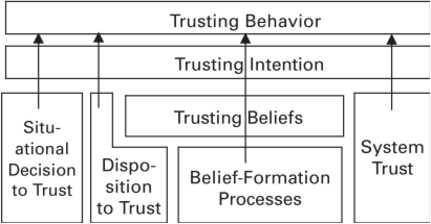
\includegraphics[width=0.5\textwidth]{liu2010RelationshipStack}
	\caption[Trust Construct Relationships]{Trust Construct Relationships (from \citet{Liu2010})}
	\label{fig:trust_constructs}
\end{figure}


\subsection{Taxonomy and Notations of Trust}\label{sec:trust_taxonomy}

To abstractly discuss Trust and trust modelling, \citet{Liu2006} present a $T\{\text{subject}:\text{agent},\text{action}\}$ notation for individual trust relationships, where \emph{Subject} and \emph{Agent} usually representing individuals but may include groups of individuals or the network as a whole, and \emph{Action} may be an action performed by a given agent or a property possessed by that agent.

This notation is normally abbreviated such that 
\begin{equation}
  \label{eq:trust_notation}
  T\{A:B,a\} = T^a_{AB}
\end{equation} 
where $T^a_{AB}$ denotes the expectation or trust that a node $A$ has that node $B$ will successfully perform action $a$.

A special extension is assumed for multi-party trust relationships for the ``action'' of recommending another nodes perspective on a given nodes expectation or trust that it will perform an action $a$; ($a_R$)
%
\begin{equation}
  \label{eq:recommendation_notation}
  T\{A:B,a_R\} = R^a_{AB}
\end{equation}
%
Where the action under discussion is implied or there is a single action under debate (for example, packet routing in \glspl{manet}), the action superscript can be left out; $T_{AB} , R_{AB}$.

Trust can be propagated through a number of nodes, forming a chain of assessments and recommendations, expressed as per \eqref{eq:trust_prop}.
While the particular algorithms and methods of combination vary between \glspl{tmf}, the $\cdot$ symbol is used as a generic operator.
In any case, if a given node $A$ has no knowledge about node $B$, or likewise $B$ having no knowledge of $C$, trust between $A,C$ is zero; $T_{ABC} = 0$

\begin{equation}
	\label{eq:trust_prop}
	T_ {AC}\mapsto T_{ABC} = R_{AB} \cdot T_{BC} \text{ where } R_{AB} \neq 0 , T_{BC} \neq 0
\end{equation}

Either notation; $T_{AC}, T_{ABC}$ is valid for this chaining depending on the context, where, $T_{AC}$ is preferred where there is either one unambiguous transiting node $B$, or where the value is the multi-path trust synthesis across many individual links, where $T_{ABC}$ is then the preferred notation for a single path within a multi-path network.

For discussion of individual links or subsets of links, Set notation can be applied to $T_{AC}$ multi-path networks based on the graph theoretic notation introduced in~\autoref{sec:manet_topologies}, for example;

\begin{equation}
	T_{AC} \subseteq T_{AxC} \forall x | \overrightarrow{AxC} \in E
\end{equation}

Similarly, these multi-path sets can be decomposed into their individual links, i.e. $T_x \ge 0 \forall x \in T_{AC}$
\subsubsection{Characteristics of Trust Relationships}

There are five commonly considered characteristics or attributes of Trust relationships in general, but not all relationships exhibit them and they are not assumed to be a complete specification of Trust (synthesised from \cite{Liu2006,Mayer1995, Mcknight1996, Pavan2015}):

\begin{itemize}
	\item \emph{Multi-Party} - One-to-one; one-to-many; many-to-one; many-to-many.
	Trust is not an absolute characteristic of a lone individual.
	Trust may include multi-agent abstractions (one-to-many), such as a preferential trust/distrust towards a group exhibiting a particular attribute, e.g.\ members of the armed forces / police services.
	Likewise, there can be trustor/trustee attributes that can generalise relationships between collectives (many-to-many), e.g.\ Jets and Sharks\cite{Robbins1961}.
	\item \emph{Transitive} - Trust assessments can be shared (i.e.\ recommendations), where this second order trust assessment incorporates both the observed trustworthiness of the trustee, as well as the trustworthiness of the intermediate trustor.
	In some models this is further extended to include out-of-network intermediate trustors that have some other defined authority, e.g.\ PKI Certificate Authority
	\item \emph{Evidential} - Trust must be based on some form of evidence-based observation or assessment, such as historical success rates of performing a certain action, or second-hand observations of trust from a third party.
	\item \emph{Directional Asymmetry} - The majority of relationships are bi-directional but are asymmetric, i.e.\ between two entities who ``trust'' each other, there are two independent trust relationships that may have very different ``values'' or extents.
	\item \emph{Contextual} - Trust can be variable and loosely coupled between contexts with respect to the action being assessed or the environment within which the trustee is operating, e.g.
	Doctors are trusted to perform medical procedures but that trust may not improve their success at correctly wiring an electrical plug.
	However there are plenty of counter-examples to this, as from \cite{Mayer1995}, two of the three listed factors of trust are ``Benevolence'' and ``Integrity'' and these are unrelated to the ability of a trustee to perform a particular action, so it is reasonable to make an initial assumption that if a trustee is being benevolent in one activity or context, that that benevolence \emph{should} extend to other contexts.
\end{itemize}

\cite{Liu2010} summarises these attributes in a series of axioms 

\subsubsection{Fundamental Axioms of Trust}\label{sec:axioms}
\citet{Sun2008} demonstrate that by taking an Information Theoretic approach to trust as function of entropy and as such, uncertainty (i.e.\ trust having both a valency and a confidence)~\footnote{Donald Rumsfelds famous 2002 ``Known Knowns'' quote is a perfect example of this}, a series of axioms can be constructed to model the interactions between trusting agents.
Many of these axioms are mirrored in pure information theory, as discussed in \cite{Liu2010}.

\emph{Axioms and their quoted descriptions from \cite{Liu2010}}

\paragraph{Axiom 1: Concatenation propagation of Trust does not increase Trust} 
\begin{displayquote}
	When the subject establishes a trust relationship with the agent through the recommendation from a third party, the trust value between the subject and the agent should not be more than the trust value between the subject and the recommender as well as the trust value between the recommender and the agent.
\end{displayquote}
This axiom sets up the rules for trust propagation from an entropic perspective and using the notation discussed above, can be expressed as in \eqref{eq:trust_prop} (see~\autoref{fig:trust_chaining} for context)
\begin{equation}
	\label{eq:trust_prop}
	T_{AC} \leq \min({R_{AB},T_{BC}})
\end{equation}



\todo{FIX: Label placements}

\begin{figure}
	\centering
	\begin{tikzpicture}[auto, node distance=1.5cm and 0.5cm, line width=2pt, >=latex']
	\node [sum, preaction={fill=red!20}] (a) {A};
	\node [sum, right =of a] (b) {B};
	\node [sum, right =of b] (c) {C};
	
	\draw [dashed, ->] (a) -- (b) node [midway] {$R_{AB}$};
	\draw [->] (b) -- (c) node [midway] {$T_{BC}$};;
	
	\end{tikzpicture}
	\caption{Trust Chaining}
	\label{fig:trust_chaining}
\end{figure}

\begin{figure}
	\centering
	\begin{subfigure}[b]{0.35\textwidth}
		\hfill
		\begin{tikzpicture}[auto, node distance=1.5cm and 0.5cm, line width=2pt, >=latex', baseline=(a.base)]
		\node [sum, preaction={fill=red!20}] (a) {A};
		\node [sum, right =of a] (b) {B};
		\node [sum, right =of b] (c) {C};
		
		\draw [dashed, ->] (a) -- (b) node [midway] {$R_\alpha$};
		\draw [->] (b) -- (c) node [midway] {$T_\alpha$};;
		
		\end{tikzpicture}
		\label{fig:trust_combination_a}
		\caption{}
		\hfill
	\end{subfigure}
	\begin{subfigure}[b]{0.35\textwidth}
		\hfill
		\begin{tikzpicture}[auto, node distance=1.5cm and 0.5cm, line width=2pt, >=latex', baseline=(a.base)]
		\node [sum, preaction={fill=red!20}] (a) {$A'$};
		\node [sum, above right =of a] (b) {$B'$};
		\node [sum, below right =of a] (d) {$D'$};
		\node [sum, below right =of b] (c) {$C'$};
		
		\draw [dashed, ->] (a) -- (b) node [midway] {$R_\alpha$};
		\draw [dashed, ->] (a) -- (d) node [midway] {$R_\alpha$};
		\draw [->] (b) -- (c) node [midway] {$T_\alpha$};;
	    \draw [->] (d) -- (c) node [near end, below] {$T_\alpha$};;
		
		\end{tikzpicture}
		\label{fig:trust_combination_b}
		\caption{}
		\hfill
	\end{subfigure}
	\caption{Trust Combination}
	\label{fig:trust_combination}
\end{figure}


\paragraph{Axiom 2: Multipath propagation of Trust does not reduce Trust}

\begin{displayquote}
	If the subject receives \textit{the same} recommendations for the agents from multiple sources, the trust value should be no less than that in the case when the subject receives fewer recommendations.
\end{displayquote}

In this case, this axiom sets the groundwork for multi-node analysis of trust networks, shown in~\autoref{fig:trust_combination} and described in \eqref{eq:trust_combination}.
In essence, adding additional information sources of the same observation should increase the trust value arrived at from a smaller subset of sources.

\begin{align}
T_{AC} \geq T_{A'C'} \geq 0, &\text{ for } R_\alpha \ge 0, T_\alpha \geq 0\\
T_{AC} \leq T_{A'C'} \leq 0, &\text{ for } R_\alpha \ge 0, T_\alpha \le 0
\end{align}


\begin{figure}
	\centering
	\begin{subfigure}[b]{0.35\textwidth}
		\hfill
		\begin{tikzpicture}[auto, node distance=1.5cm and 0.5cm, line width=2pt, >=latex', baseline=(a.base)]
		\node [sum, preaction={fill=red!20}] (a) {A};
		\node [sum, right =of a] (b) {B};
		\node [sum, below right =of b] (e) {E};
		\node [sum, above right =of b] (d) {D};
		\node [sum, below right =of d] (c) {C};
		
		\draw [dashed, ->] (a) -- (b) node [midway] {$R_{AB}$};
		\draw [dashed, ->] (b) -- (e) node [midway] {$R_{BE}$};
		\draw [dashed, ->] (b) -- (d) node [midway] {$R_{BD}$};
		\draw [->] (e) -- (c) node [midway] {$T_{EC}$};;
		\draw [->] (d) -- (c) node [near end, below] {$T_{DC}$};;
		
		\end{tikzpicture}
		\label{fig:trust_paths_a}
		\caption{}
		\hfill
	\end{subfigure}
	\begin{subfigure}[b]{0.35\textwidth}
		\hfill
		\begin{tikzpicture}[auto, node distance=1.5cm and 0.5cm, line width=2pt, >=latex', baseline=(a.base)]
		\node [sum, preaction={fill=red!20}] (a) {$A'$};
		\node [sum, above right =of a] (b) {$B'$};
		\node [sum, right =of b] (d) {$D'$};
		\node [sum, below right =of a] (f) {$F'$};
		\node [sum, right =of f] (e) {$E'$};
		\node [sum, below right =of d] (c) {$C'$};
		
		\draw [dashed, ->] (a) -- (b) node [midway] {$R_{A'B'}$};
		\draw [dashed, ->] (a) -- (f) node [midway] {$R_{A'F'}$};
		\draw [dashed, ->] (f) -- (e) node [midway] {$R_{F'E'}$};
		\draw [dashed, ->] (b) -- (d) node [midway] {$R_{B'D'}$};
		\draw [->] (e) -- (c) node [near end, below] {$T_{E'C'}$};
		\draw [->] (d) -- (c) node [near end, above] {$T_{D'C'}$};
		
		\end{tikzpicture}
		\label{fig:trust_paths_b}
		\caption{}
		\hfill
	\end{subfigure}
	\caption{Trust Paths}
	\label{fig:trust_paths}
\end{figure}

\paragraph{Axiom 3: Trust based on multiple recommendations from a single source should not be higher than that derived from independent sources.}

\begin{displayquote}
	When the trust relationship is established jointly through concatenation and multipath trust propagation, [...] recommendations from independent sources can reduce uncertainty more effectively than can recommendations from correlated sources.
\end{displayquote}

This axiom addresses the information independence of trust links; In ~\autoref{fig:trust_paths} there are two networks, both with two potential chains from right to left-nodes ($A,C,A',C'$),.
\begin{align}
T_{AC}&=\{T_{ABCD}, T{ABEC}\}\\
T_{A'C'}&=\{T_{A'B'D'C'}, T{A'F'E'C}\}
\end{align}

Given that the sub-chain $T_{AB}$ prepends both chains in $T_{AC}$, the weight of node $B$'s recommendations are effectively duplicated, and from Axiom 2, this duplication should not decrease the trust assessment.
However for $T{A'C'}$, no such duplication exists, and as such it's trust assessment should have a larger magnitude.

\begin{align}
T_{AC} \geq T_{A'C'} \geq 0, &| T_{A'C'} \geq 0\\
T_{AC} \leq T_{A'C'} \leq 0, &| T_{A'C'} \le 0
\end{align}


\subsection{Topologies of Multi-Party Trust Networks}\label{sec:trust_topologies}
Beyond the attributes or characteristics of an individual trust relationship, within any multi party sparsely connected network or community, topological context is useful in both establishing trust and in disseminating observations for collaborative assessment.

Within sparsely connected networks, there are three primary types of relationship, minimally demonstrated in Fig.~\ref{fig:trust_topology_relationships};

\begin{itemize}
  \item \emph{Direct} - Whereby two nodes have a 1-hop communications link between them ($A,B,C$ in the given figure)
  \item \emph{Indirect} - Where two nodes have a $n>1$ hop communications link ($E,D$ from $A$ or $C$s perspective in the given figure), i.e.\ there is no direct link from the trustor ($A$) to trustees ($E,D$)
  \item \emph{Recommendation} -  Where three nodes are fully connected so as to enable the exchange of direct opinions and form composite opinions based on the target and reporter (i.e.\ $A$ has both its own Direct assessment of $C$, as well as it's knowledge of $B$s Direct assessment of $C$)
\end{itemize}

\begin{figure}
  \centering
  \begin{subfigure}[t]{0.40\textwidth}
    \hfill
    \begin{tikzpicture}[auto, node distance=1.5cm and 0.5cm, line width=2pt, >=latex']
      \node [sum, preaction={fill=red!20}] (a) {A};
      \node [sum, below left =of a] (b) {B};
      \node [sum, below right =of a] (c) {C};
      \node [sum, below left =of c] (d) {D};
      \node [sum, above right =of c] (e) {E};
      \node [sum, below right =of c] (f) {F};

      \graph{
      (a) -- (b);
      (a) -- (c);
      (b) -- (c);
      (b) -- (d);
      (c) -- (d);
      (c) -- (e);
      (c) -- (f);
      };

      \begin{pgfinterruptboundingbox}
        \coordinate (A) at (a);
        \cercle{A}{2.25cm}{216}{160}{1.50}{red, opacity=0.5, dashed};
      \end{pgfinterruptboundingbox}
    \end{tikzpicture}
    \caption{Sample topology showing logical connections between nodes (Range of $A$ shown in red dashed line)}
    \hfill
  \end{subfigure}

  \begin{subfigure}[t]{0.25\textwidth}
    \begin{tikzpicture}[auto, node distance=1.5cm and 0.5cm, line width=2pt, >=latex']
      \node [sum, preaction={fill=red!20}] (a) {A};
      \node [sum, below left =of a] (b) {B};
      \node [sum, below right =of a] (c) {C};
      \node [sum, below left =of c] (d) {D};
      \node [sum, above right =of c] (e) {E};
      \node [sum, below right =of c] (f) {F};


      \graph[edges={opacity=0.4}]{
      (a) -- (b);
      (a) -- (c);
      (b) -- (c);
      (b) -- (d);
      (c) -- (d);
      (c) -- (e);
      (c) -- (f);
      };

      \draw[->, blue, dashed] (a) to[bend right] (b) node [left of=a] {$T_{A,B}$};
      \draw[->, purple, dashed] (a) to[bend left] (c) node [right of=a] {$T_{A,C}$};

    \end{tikzpicture}
    \caption{Direct Relationships, the two possible trust assessments from $A$ to its connected neighbours, $B,C$}
  \end{subfigure}
  \hfill
  \begin{subfigure}[t]{0.25\textwidth}
    \begin{tikzpicture}[auto, node distance=1.5cm and 0.5cm, line width=2pt, >=latex']
      \node [sum, preaction={fill=red!20}] (a) {A};
      \node [sum, below left =of a] (b) {B};
      \node [sum, below right =of a] (c) {C};
      \node [sum, below left =of c] (d) {D};
      \node [sum, above right =of c] (e) {E};
      \node [sum, below right =of c] (f) {F};


      \graph[edges={opacity=0.4}]{
      (a) -- (b);
      (a) -- (c);
      (b) -- (c);
      (b) -- (d);
      (c) -- (d);
      (c) -- (e);
      (c) -- (f);
      };

      \draw[->, blue, dashed] (a) to[bend right] (c.west) to [bend right](d.north east) node [right of=d] {$T_{A,C,D}$};
      \draw[->, purple, dashed] (a) to[bend left] (b.east) to [bend left](d.north west) node [left of=d] {$T_{A,B,D}$};
      \draw[->, teal, dashed] (a) to[bend left] (c.north east) to [bend left](e.west) node [above of=c] {$T_{A,C,E}$};
      \draw[->, magenta, dashed] (a) to[bend left] (c.north) to [bend left](f.north) node [right of=c] {$T_{A,C,F}$};
    \end{tikzpicture}
    \caption{Indirect Relationships, showing the four possible trust assessments from $A$ or the three disconnected leaf nodes, $D,E,F$}

  \end{subfigure}
  \hfill
  \begin{subfigure}[t]{0.25\textwidth}
    \begin{tikzpicture}[auto, node distance=1.5cm and 0.5cm, line width=2pt, >=latex']
      \node [sum, preaction={fill=red!20}] (a) {A};
      \node [sum, below left =of a] (b) {B};
      \node [sum, below right =of a] (c) {C};
      \node [sum, below left =of c] (d) {D};
      \node [sum, above right =of c] (e) {E};
      \node [sum, below right =of c] (f) {F};


      \graph[edges={opacity=0.4}]{
      (a) -- (b);
      (a) -- (c);
      (b) -- (c);
      (b) -- (d);
      (c) -- (d);
      (c) -- (e);
      (c) -- (f);
      };

      \draw[->, blue, dashed] (a) to[bend right] (b) node [left of=a] {$T_{A,B}$};
      \draw[->, purple, dashed] (a) to[bend left] (c) node [right of=a] {$T_{A,C}$};

      \draw[->, blue, dashed] (a) to[bend left] ([yshift=5pt] c.north west) to [bend right](b.east)  node [above left of=d, xshift=2ex, yshift=-3ex] {$T_{A,C,B}$} ;
      \draw[->, purple, dashed] (a) to[bend right] ([yshift=5pt] b.north east) to [bend left](c.west) node [above right of=d, xshift=-2ex, yshift=-3ex] {$T_{A,B,C}$};

    \end{tikzpicture}
    \caption{Recommender Relationship, showing the two discrete paths trust assessments travel to $A$; $T_{A,B}^R = T_{A,C} \cdot T_{C,B}$ and  $T_{A,C}^R = T_{A,B} \cdot T_{B,C}$}

  \end{subfigure}
  \hfill
  \caption{Trust Topologies; Direct, Indirect, Recommender, etc.\ from the perspective of Node A}
  \label{fig:trust_topology_relationships}
\end{figure}

\subsection{Trust Establishment Strategies}

\todo{ADD: Need to discuss how trust is established a) initially among a co-launched group, b) with a newcomer and c) with a returner (\citet{Liu2006, Li2007, Theodorakopoulos2004})}

\subsection{Attacks on Trust}

\citet{Liu2010} identify four types of attacks on Trust within networks that generate collaborative trust assessments through the exchange of recommendations; On-Off, Conflicting-behaviour, Badmouthing, and Sybil/Newcomer attacks.

\begin{enumerate}
	\item \emph{Bad Mouthing:} Where a malicious node provides dishonest recommendations of other nodes in the network, to disrupt optimal operation  by making other nodes appear untrustworthy
	\item \emph{Sybil attack:} Where a malicious node uses multiple pseudonymous entities to diffuse blame for bad behaviour, while maintaining a good reputation using the nodes genuine identity
	\item \emph{Newcomer Attack:} Similar to the Sybil attack in operation, whereby a malicious node will periodically assume a ``fresh'' identify with the network, shedding an identity that as accumulated an ``untrustworthy'' assessment
	\item \emph{Conflicting Behaviour attack:} Where a node (or a collaborating collection of malicious nodes) selectively drops messages, or modified recommendation values to or from certain nodes or groups of nodes, implicitly reducing the apparent trustworthiness of those attacked nodes with the rest of the fleet, while reducing the operational efficiency of the fleet overall.  This attack exploits the dynamic properties of trust through taking advantage of the expected dynamism in topology and behaviors such that other nodes ``won't notice'' (Alternatively called the Grey Hole Attack)
	\item \emph{On-Off attack:} Malicious entities alternate between ``good'' and ``bad'' behaviours, hoping that they can remain undetected while causing damage. This attack exploits the dynamic properties of trust through time-domain inconsistent behaviours.
\end{enumerate} 

It is to be noted that the Sybil and Newcomer attacks do not exclusively rely on trust, but instead are a problem of network authentication.

The all of these attacks can be abstracted as ``non-isotropic attacks'' i.e.\ attacks that attempt to hide malicious / selfish behaviour behind the expected statistical variation in observations within a cohort.
In each case, a different dimension of this assumed statistical normality is exploited; in On-Off, the attacker attempts to ``hide'' in the time dimension by only occasionally misbehaving, in the Badmouth attack the attacker is relying on it's false recommendation being equitably received as its targets true actions. 
In the Conflicting behaviour attack, the attacker effectively ``badmouths'' a subset of nodes, hiding itself amid the ``false'' reports coming from the conflicting subsets of nodes. 
Finally, in Sybil/Newcomer attacks the attacker takes advantage of an assumed naivety of the collective by presenting itself as a ``new'', and therefore, zero-history entity that can initially neither be trusted nor untrusted.\todo{FIX: Backref to ``Trust vs UnTrust'' section}


\section{Trusted Development and Operation of Autonomous Systems}\label{sec:trust_autonomy}

\subsection{Introduction}

The aim of the section is to explore where trust is likely to impact \gls{sos} that contain autonomous elements incorporating Human Factors, Command and Control considerations, and \gls{v2v} distributed communication, from the perspective of trusted and semi-trusted operation.

\todo{ADD:Expand introduction and plan the rest of the section}

\subsection{Autonomy and Levels of Autonomy}

Autonomy, like trust, is a nebulous term applied across research, defence and commercial circles that has its origins in human experience and interactions. 

Autonomy, coming from the Greek roots \textit{auto-} (self) and \textit{nomos} (law) is the concept of a self-driven agency, and can be considered the concept of a ``rational'' individuals capacity to make un-coerced decisions in an informed manner. 
This autonomy is distinct from \textit{freedom}, where freedom is the \textit{ability} to perform an action, not the \textit{capability to choose} which action to perform.
That is not to say that autonomy or autonomous action exists in an ideal vacuum with perfect and complete information with no coercive factors or outside influences.
The ability to recognise, process, weight and filter inputs, knowledge, ``responsibilities'', influences and outside factors and come to an effective decision is a key skill for any self-governing agent, however this is above and beyond the concept of ``basic autonomy''.
From the implicit variability and complexity of environment and context that classically autonomous entitie\footnote{That's \textit{Homo Sapiens}} inhabit, there is little assumption that ``autonomy'' always produces a categorically ``correct''or ``good'' decision, but is instead a case of an agent choosing the action that is \textit{in its own best interests based on available information}\cite{Arpaly2003}.\footnote{Arply discusses a counter example of this ``goodness'' assessment as  Huckleberry Finns' release of Jim against his ``best judgement'', and that rather than this action being an instance of morally justified or self-congratulatory autonomy, it was ``the right thing to do'' from an abstract moralistic perspective rather than a justifiably beneficial action, and it is a case of \textit{akrasia}; the lacking of self-governance and the antonym of autonomy.}

This understanding of individual autonomy has been scaled up through social systems and has been studied at length to understand the emergence of post-Marxist proto-anarchistic movements~\cite{Hunter2016} and from a higher perspective, international politics, especially in the cases of quasi-federalised collections of states such as the United States of America~\cite{Halberstam2001} and the European Union/Eurozone/Schengen Area~\cite{Richter2012}


In the most general case in the world of artificial systems, Autonomy is understood as a graduated spectrum of allocation of functionality between a system (or system of systems) and a human operator assigned with performing a given task. 
Where a system is more ``autonomous'', more of the sensing, planning, decision and action operations are performed by the system. (See Table~\ref{tab:autonomy_definitions} for a review of current definitions of autonomy and autonomous systems)
This graduated spectrum of allocated functionality is generally termed the \gls{loa}, where an increasing \gls{loa} correlated to increasing control and decision making freedom to the autonomous system from the human operator(\autoref{tab:autonomy_levels_sheridan}).
These levels can be loosely viewed as a spectrum from across Planning Support, Decision Support, Bounded Execution, and finally, Informed Execution\footnote{In theory there is a further ``Uninformed execution'' level of autonomy, however this is beyond the scope of this work\cite{Cameron1984}}.

While Autonomy is largely taken to be a robotics term based in the case of one human operator and one robotic entity, the development of more generalised cyber-physical systems has expanded this definition; from over-the-horizon human operation of \glspl{uav} to global networks of collaborating machines such as Google and beyond.

As such, the interactions \emph{between} autonomous agents are becoming increasingly relevant to the operating efficiencies of overall collaborative systems, wether or not a human operator is ``in-the-loop''.

See \autoref{apx:human_factors} for a more thorough discussion on the Human Psychological Factors related to the planning, use, and integration of trusted autonomous systems in classical command and control contexts.


\begin{table}\centering
  \caption{Definitions of Autonomy}
  \label{tab:autonomy_definitions}
  \begin{tabularx}{\textwidth}{X p{3cm}}\toprule
    Definition & Source \\ \midrule
    \ldots should be able to carry out its actions and to refine or modify the task and its own behaviour according to the current goal and execution context of its task & \citet{Alami1998}\\
    Autonomy refers to systems capable of operating in the real-world environment without any for of external control for extended periods of time & \citet{Bekey2005}\\
    \ldots a system situated within and a part of an environment that senses that environment and acts on it, over time, in pursuit of its own agenda and so as to effect with it senses in the future. \ldots Exercises control over its own actions & \citet{Franklin1997} \\
    An unmanned systems own ability of sensing, perceiving, analysing, communicating, planning, decision-making, and acting, to achieve goals as assigned by its human operator(s) through designed \gls{hri}. \ldots The condition or quality of being self-governing & \citet{Huang2004}\\
    \ldots that the robot can operate self-contained, under all reasonable conditions without requiring recourse to the human operator. Autonomy means that a robot can adapt to change in its environment \ldots or itself \ldots and continue to reach a goal. & \citet{Murphy2000}\\
    \ldots it should learn what it can to compensate for partial or incorrect prior knowledge & \citet{Russell2009} \\
    Autonomy refers to a robot's ability to accommodate variations in its environment. Different robots exhibit different degrees of autonomy; the degree of autonomy is often measured by relating the degree at which the environment can be varied to the mean time between failures and other factors indicative of the robots performance. & \citet{Thrun2004}\\
    \ldots agents operate without the direct intervention of humans or others, and have some kind of control over their actions and internal states. & \citet{Wooldridge1995}\\
    Systems have a set of intelligence based capabilities or learning adaptive capabilities that allow it to respond within a bounded domain to situations that were not pre-programmed or anticipated in the design. & \citet{Fox2014}\\\bottomrule
  \end{tabularx}
\end{table}

\begin{table}\centering
  \caption[Levels of Decision Making Automation]{Levels of Decision Making Automation (Extended from \citet{Sheridan1978})}
  \label{tab:autonomy_levels_sheridan}
  \begin{tabularx}{\textwidth}{c c X}\toprule
    \gls{loa} & Description \\ \midrule
    1&    The computer offers no assistance; the human must make all decisions and actions\\
    2&    The computer offers a complete set of decision/action alternatives, or\\
    3&    Narrows the selection down to a few, or\\
    4&    Suggests one alternative and\\
    5&    Executes that suggestion if the human operator approves, or\\
    6&    Allows the human a restricted time to veto before automatic execution, or\\
    7&    Executes automatically, then necessarily informs the human, and\\
    8&    Informs the human only if asked, or\\
    9&    Informs the human only if it, the computer, decides to.\\
    10&   The computer decides everything and acts autonomously, ignoring the human.\\\bottomrule
  \end{tabularx}
\end{table}
%\todo{Ref \autoref{tab:autonomy_levels_sheridan} there may be a case to discuss the breakdown of ``Plan, Decide, Execute, Inform'', possibly a nice onion-style graphic}

\begin{table}\centering
  \caption[Levels of Automation]{Levels of Automation (paraphrased from \citet{Endsley1999})}
  \label{tab:autonomy_levels_endsley}
  \begin{tabularx}{\textwidth}{p{3cm} X}\toprule
    \gls{loa} & Description \\ \midrule
    Manual Control &
    The human monitors, generates options, selects options (makes decisions), and physically carries out options.\\
    Action Support &
    The automation assists the human with execution of selected action. The human does perform some control actions.\\
    Batch Processing &
    The human generates and selects options; then they are turned over to automation to be carried out (e.g., cruise control in automobiles)\\
    Shared Control &
    Both the human and the automation generate possible decision options. The human has control of selecting which options to implement; however, carrying out the options is a shared task.\\
    Decision Support &
    The automation generates decision options that the human can select. Once an option is selected, the automation implements it.\\
    Blended Decision Making & 
    The automation generates an option, selects it, and executes it if the human consents. The human may approve of the option selected by the automation, select another, or generate another option.\\
    Rigid System &      
    The automation provides a set of options and the human has to select one of them. Once selected, the automation carries out the function.\\
    Supervisory Control &
    The automation selects and carries out an option. The human can have input in the alternatives generated by the automation.\\
    Automated Decision Making & 
    The automation generates options, selects, and carries out a desired option. The human monitors the system and intervenes if needed (in which case the level of automation becomes Decision Support).\\
    Full Automation &   The system carries out all actions.\\ \bottomrule
  \end{tabularx}
\end{table}


\subsection{Trust Perspectives in Autonomous Operation}\label{sec:trust_perspectives}

For the purposes of this work, two perspectives on trust for autonomous systems are defined: Design Trust and Operational Trust.

\begin{itemize}
  \item \emph{Design Trust} - When an autonomous system is under development a level of Trust is established in it through the manner in which it has been designed and tested.
    This is the same as conventional systems.
    Given that systems that have high-levels of autonomy are designed to behave adaptively to dynamic environments, it is challenging to fully predict such non-deterministic behaviours prior to operational deployment.
    For example, in a navigation system it is difficult to predict the dynamic environment it will need to adapt to.
    Trust needs to be developed so that the design and testing of such systems are sufficient to predict that operation will be, if not optimal, at least satisfactory.

  \item \emph{Operational Trust} - Trust at runtime or in-situ that both the individual nodes within a system are operating as expected and that the interfaces between the operator and the system are as expected.
    This latter aspect covers issues such as physical/wireless links and interpretation of data at each end of such a communication link.
    Can be subdivided into two types of perspective;
    \begin{itemize}
      \item \emph{Hard Trust} or technical trust - The quantitative measurement and communication of the expectation of an actor performing a certain task, based on historic performance and through consensus building within a networked system.
    Can be thought of as a de-risking strategy to measure and monitor the ability of a system, or another actor within a system, to perform a task unsupervised.
  \item \emph{Soft Trust} or common trust - The qualitative assessment of the ability of an actor to perform a task or operation consistently and reliably based on social or experiential factors.
    This is the ‘human’ form of trust and is the main motivational driver for the human-factors trust discussion in \autoref{apx:human_factors}.
    Can be viewed as the abstract level of confidence an operator has in an actor to perform a task unsupervised.
    \end{itemize}
\end{itemize}

Operational Trust is functionally derived from, but distinct from Design Trust.

It is already clear that these two definitions are extremely close in their construction, but represent fundamentally different approaches to trust, one coming from a sociological perspective of person-to-person and person-to-group relationships from day to day life, and the other coming from a statistical or formal appraisal of an operation by a system.

\todo{ADD:Need to provide a linking section to the next blocks about Design/Operational Trust}


\subsection{Design Trust}\label{sec:design_trust}

As part of \cite{Bolster2014a}, five aspects of Design Trust have been identified, with major questions in each respective aspect emphasised.

\begin{enumerate}
  \item \textbf{Formal Specification of Dynamic Operation}: Autonomous Systems (AS) may be required to operate in complex, uncertain environments and as such their specification may need to reflect an ability to deal with unspecified circumstances.
    This includes engaging with dynamic systems of systems environments where an autonomous system may cooperate with a system not envisaged at design time.
    \textit{How can systems that are required to demonstrate that they meet their requirement be specified flexibly enough to permit adaptive behaviours}?
  \item \textbf{Security}: Any unmanned system has the potential to be used for illegitimate purposes by unscrupulous third parties who could exploit security vulnerabilities to gain control of the system or sub-systems.
    Any system that has the potential to cause harm from such actions must have security designed in from the start to ensure that the system can be trusted to be resilient from cyber attack.
    Current accreditation schemes rely on a security assessment of a known architecture and there are mutual accreditation recognition schemes that could be encoded in dynamic discovery handshake protocols.
    This would produce a secure network assured through the accreditation of its component systems.
    For example, the Multinational Security Accreditation Board (MSAB) deals with Combined Communications Electronics Board (CCEB) and NATO Accreditations to provide security assurance of internationally connected networks.
    Encoding such agreements into secure handshakes could enable dynamic accreditation of autonomous systems cooperating in a coalition environment.
    It is not known whether these have been demonstrated, so the question is: \textit{Can autonomous systems be designed to understand the security situation when interfacing with known or unknown systems?}
  \item \textbf{Verification and Validation of a Flexible Specification}: Following on from the description of a flexible specification, establish that the AS conforms and performs in accordance to the specification.
    This has direct implication for the trust in the resultant system.
    How can systems demonstrate that they will behave acceptably when the environment is unknown?
  \item \textbf{Trust Modelling and Metrics}: This could be argued as part of the Verification and Validation of the system.
    However, models are increasingly being embedded into system design as a reference.
    Thus it is useful to consider this element separately.
    \textit{How can trust be modelled sufficiently to span the space of most potential behaviours to help ensure that systems will be trusted when moved into operational environments?
    Can this be measured to allow comparison and minimum requirements set?}
  \item \textbf{Certification}: The certification requirements placed on specific systems will vary depending on domain and national approaches to certification.
    However, the common element in the requirement for certification is that a certified system is deemed as sufficiently trustworthy for use within its context of certification.
    Additionally Certification also relies on the predictability of a system.
    Because the aim of autonomous systems is to deal effectively with uncertain environments, \textit{can they (autonomous systems) be certified without being demonstrated in the environment within which they will adapt new behaviour?}
\end{enumerate}

While this work is primarily concerned with those aspects of \textbf{Trust Modelling and Metrics}, it is useful to consider this Trust assessment in the wider context of the design process, and what best practices are available.
Design against and Compliance with existing standards can contribute significantly to the demonstrable trustworthiness of any systems’ design.
If a system has been designed to a Standard then it has known properties that have been accepted as good practice.
However, current standards do not address the issue of the five areas listed above.

There are three main organisations that are developing or have developed assurance standards for Unmanned Systems in commercial, civil and military applications:

\begin{itemize}
  \item NATO Standardization Office (NSO)
  \item \acrfull{sae}
  \item \acrfull{astm}
\end{itemize}

\paragraph{NATO Standardization Office}
Faced with the growing adoption of similar but disparate \gls{uav} systems within NATO territories and coalition nations, STANAG 4586\cite{STANAG4586} was promulgated in 2005 and defined a logistic and interoperability framework to provide commonality in the command and control architecture and implementations of \gls{uav}/Ground station communications.

This included a particularly interesting development in the form of \gls{sae} \gls{vsm} interoperability, whereby existing systems could be grandfathered into STANAG 4586 compliance by the addition of a \gls{vsm} to operate as a protocol translator.
This \gls{vsm} could be mounted on the remote system directly, utilising a compliant \gls{dli}, or mounted on the ground-based controller, retaining the proprietary \gls{dli} to the remote system.
The standard describes five \acrfull{loi} for compliant \gls{uav} systems, shown in Table~\ref{tab:levels_of_interoperability}.
This structure has been criticised as being short sighted and at odds with the reality of modern and proposed autonomous vehicle operations \cite{Cummings2010}, specifically that in modern autonomous systems, there is no such thing as ``direct control'' or ``Operator-in-the-loop'', especially in the case of \gls{blos} systems, and that in increasingly autonomous systems, operation is done as \gls{hsc}, or more commonly described as ‘Operator-on-the-loop’, whereby the operator interacts with the intermediate autonomous system and that autonomous system eventually performs that task on the hardware.

\begin{table}
  \begin{tabularx}{\textwidth}{lX}
    \toprule
    \gls{loi} &  Description\\ \midrule
    1 &  Indirect receipt/transmission of \gls{uav} related payload data\\ 
    2 &  Direct receipt of \gls{isr} data where “direct” covers reception of \gls{uav} payload data by the UCS when it has direct communication with the \gls{uav}\\ 
    3 &  Control and monitoring of the \gls{uav} payload in addition to direct receipt of \gls{isr}/other data\\ 
    4 &  Control and monitoring of the \gls{uav}, less launch and recovery\\
    5 &  Launch and Recovery in addition to \gls{loi} 4\\ 
    \bottomrule 
  \end{tabularx}
  \caption[\gls{loi} for STANAG 4586 Compliant UCS]{Levels of Interoperability for STANAG 4586 Compliant UCS \cite{STANAG4586}}
  \label{tab:levels_of_interoperability}
\end{table}

Further, the standard predominantly deals with a one-to-one mapping between operators and nodes, when this is quite against the current state of the art; greater focus is being made in collective and collaborative assignment and having a single operating agent managing groups of autonomous nodes in-field, and handing off vehicle management responsibilities to the individual nodes.

\paragraph{\gls{sae}}

The AS-4 steering group is responsible for the development and maintenance of the \gls{jaus} standards, which provide several service sets for Inter-System cooperation and interoperability, either in the form of a specified design language (JSIDL\footnote{\gls{jaus} Service Interface Definition Language}) or as a direct framework implementation, such as the \gls{jaus} Mobility, Mission Spooling, Environment Sensing, or Manipulator Service Sets\footnote{SAE AS6009, AS 6062, AS 6060, and AS 6057 respectively}.
This provides a stack-like interoperability model akin to the OSI inter-networking standard, providing logical connections between common levels across devices regardless of how subordinate layers are implemented.
Importantly, \gls{jaus} service models are open-sourced under the BSD-license, and a development toolkit is available for anyone to develop \gls{jaus}-compatible communications and control protocols\cite{JTS}.

It is also important to note that \gls{jaus} is part funded, and heavily utilised by, US Army and Marine Robotic Systems Joint Project Office (RS-JPO), which manage the development, testing, and fielding of unmanned (ground) systems for those respective forces.\cite{JTS,Huang2004}
This includes now legacy M160 mine clearance platform and the highly popular (both with forces and their in-field operators) iRobot Packbot inspection and \gls{eod} family of robotic platforms.

\paragraph{\gls{astm}}

The \gls{astm} F38 committee has developed a \gls{los}, single-asset-single-operator stove-piped framework for Unmanned Air Systems that is too constrained in scope for applicability to a more heterogeneous operating environment\cite{AmericanSocietyofTestingandMaterials2007}.
However, the F41 Committee, focused on \glspl{umvs} has collectively developed a range of interoperable standards, covering Communications, Autonomy and Control, Sensor Data Formats, and Mission Payload Interfacing.
Of particular interest is the Autonomy and Control standard which highlighted a requirement on the vehicle system to be able to recognise an authorised client, be that a human operator or an additional collaborating vehicle~\cite{AmericanSocietyofTestingandMaterials2006}.
Further, the standard states that the responsibility of the safety and integrity of any payload remains with the vehicle.
This standard was withdrawn in 2015 due to \gls{astm} regulations requiring standards to be updated within 8 years of approval, and has no direct replacement within \gls{astm}, but stands as a useful guiding perspective on autonomy standards within industry.

\begin{figure}
  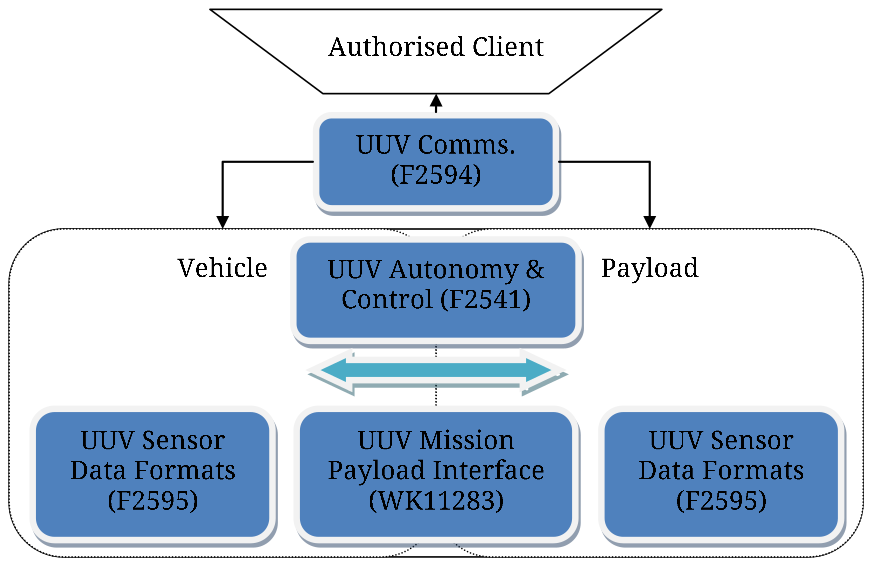
\includegraphics[width=\textwidth]{astmf41arch}
  \caption[\acrshort{astm} F41 \acrshort{umvs} Architecture]{\acrshort{astm} F41 \acrshort{umvs} Architecture  (with relevant substandards in parenthesis)}
  \label{fig:astmf41arch}
\end{figure}

\subsubsection{Summary of Design Trust}

The implications of trust in autonomy beyond securing communications and data are an area in need of further research.
Of particular concern is the verification of autonomous behaviours and failsafe behaviour~\cite{BAESystems2013}.
The addition of increased on-board autonomy in MUxS, properly understood and verified, would greatly improve this future capability, similar to recent developments in the \gls{umvs} arena~\cite{Cummings2010}.

There are opportunities for increased decentralisation and in-field collaboration~\cite{Walton2012}, however, difficulties in ``Trust'' between human operators and autonomous systems have already been clearly identified~\cite{Chen2011b},and this has been demonstrated by the recent decision by the German government to renege on its \euro500M investment in the Euro Hawk programme, due to concerns about civil certification of the onboard autonomy~\cite{Mehta2013}
In order for these new distributed structures to be relied upon to provide operational performance, reliability and to maintain in-field situational awareness, vulnerabilities to disruption, interruption, and subversion need to be understood and minimised.

\subsection{Operational Trust}

\subsubsection{Summary of Human Factors impacting Operational Trust in Defence Contexts}

When dealing with human supervision of autonomous or semi-autonomous systems, there is an inherent conflict between the expectations of the operator, and the hopes of system architects.
System architects aim to provide more and more information to the operator to justify a systems operation, and Operators in reality need less and less information to be efficient when things are going well, and responsive in a dynamic environment.
This places huge demands on Human Interface design and indeed on communications design to provide this timely, relevant, interactive connection between any autonomous system and the end operator(s).
Recent work has presented the idea of taking user interface inspiration from the entertainment sector, in terms of UI best practises developed over two decades of Real-Time Strategy game development~\cite{Johnson2007}, and follow up work into automated mission debrief demonstrated that such operational support could improve causal situational awareness of an operator when compared to a human-baseline~\cite{Johnson2011}.
In terms of the human factors challenges \footnote{See~\autoref{apx:human_factors} for a discussion of these challenges}, they are often contradictory in their direction, particularly when contrasting between Adaptive Automation and Cognitive Biases challenges.
This is a key part of the ``soft trust'' perspective, where the operators and commanders need to be able to implicitly and explicitly trust the operation of a remote system with limited feed-back bandwidth, high latency, or long-term operation such that direct remote operation is infeasible or undesirable.
To be able to trust that system's ability to continue on a course, survey an area, notify on detection of an anomaly, etc.is going to be the corner stone of any autonomous systems justification in the future.

\subsection{Summary}

\todo{ADD: Conclusion of Trusted Development}


\section{Trust in Autonomous \glspl{manet}}\label{sec:trust_manets}

\subsection{Trust Model Design Considerations}\label{sec:trust_model_design_considerations}

From the previous sections, Trust can be redefined as ``the level of confidence one agent has in another to perform a given action on request or in a certain context''.
Trust in the autonomous or semi-autonomous realm is the ability of a system to establish and maintain this level of confidence in itself or another systems' operations.

There are five topics that are important to address in any \glspl{manet} trust model~\cite{Kamvar2003}:
%
\begin{itemize}
  \item The trust model should be without infrastructure.
    Because the network routing infrastructure is formed in an ad-hoc fashion, the trust management can not depend on, e.g., a \acrfull{ttp}.
    There is no \gls{pki}, where some center nodes monitor the network, and publish illegal nodes periodically.
    In a \gls{manet}, there are no certification authorities (CA) or registration authorities (RA) with elevated privileges etc.
  \item The trust model should be anonymous because of the anonymity of mobile nodes in \glspl{manet}.\todo{Q: This isn't actually explained or justified in Kamvar so it may have been pulled out of his ass}
  \item The trust model should be robust.
    That is, it can be robust to all kinds of unfriendly attacks and the network itself should not be susceptible to attacks by unfriendly nodes.
    Moreover, in the presence of malicious nodes, they may attempt to subvert the model in order to get an unfairly good trust value.
  \item The trust model should have minimal control overhead in accordance with computation, storage, and complexity.
  \item The trust model should be self-organized.
    \glspl{manet} are characterized to have dynamic, random, rapidly changing and multi-hop topologies composed of variably bandwidth-constrained links
\end{itemize}
%

\subsection{Vulnerabilities of \glspl{manet}}

The openness of the \gls{manet} architecture leaves it inherently vulnerable to security threats. 
Mitigation protocols must be built on top of this architecture to maintain security and reliability in the face of open-access threats (whether these threats be directed attacks, uncooperative or selfish operation, or indeed malfunctioning/failing nodes).
It is worthwhile to briefly summarise the factors of \gls{manet} architecture that make it vulnerable to different threat vectors, establish the inter-node threat surface within an operating \gls{manet}.

\subsubsection{Exposed Threat Surfaces}
\emph{This section based on a summary of \citet{csen2010security} and other sources directly cited}

\emph{Wireless Links} - The use of wireless interfaces expose such networks eavesdropping and active interference, with no physical access required.
These links normally have significant channel access and bandwidth constraints compared to closed-wired networks.
This presents outside threats with the ability to eavesdrop or actively interfere with the operation of the network, leading to data security risk and risk of \gls{dos}-style attacks.

\emph{Mobility and Dynamic Topology} - Nodes joining/leaving/re-joining the network and moving around the environment leads to significant topology and access control changes, making it difficult to differentiate between malicious and normal behaviour.
Additionally this assumption of node mobility and ``temporary disconnection'' presents opportunities to outside attackers to physically compromise, capture or replicate nodes.

\emph{Assumption of Cooperation} - \gls{manet} routing is predicated on the assumed ``fairness'' of nodes both in their routing operation and their ``advertisement'' of routing capability, leading to opportunities to disrupt the optimal operation of the network\cite{Papadimitratos2002}.

\emph{Resource Constraint} - In \glspl{manet}, more than in static wired networks, secondary resources such as power, and tertiary resources such as locomotion, onboard processing and data storage capabilities present additional opportunities for selfish or malicious threat that simultaneously constrain the ability of nodes to mitigate threat (i.e. limited processing power restricting the use of advanced cryptographic protocols, power/locomotion constraints limiting the available operational time to ``learn'' about attack characteristics, etc.)

\emph{Insecure/Fuzzy Operational Boundary} - With no hard boundary between ``in network'' and ``out of network'', \gls{manet} security must combat both internal and external threats.



\begin{table}
  \caption[Selected Attacks on the Protocol Stack]{Selected Attacks on the Protocol Stack extended from \cite{csen2010security}}
  \label{tab:stack_attacks}
  \begin{tabularx}{\textwidth}{p{5cm} X}\toprule
    Layer & Attacks\\\midrule
    Application & Data Corruption, Malware, Virii and Worms\\
    Transport & SYN Flodding, Session Hijacking\\
    Network & ``HELLO'' Flood, (Black/Worm/Sink)hole, Sybil, Replay, Rishing, Resource-Consumption\\
    Data Link & Monitoring, Traffic Analysis\\
    Physical& Eavesdropping, Active Interference\\\bottomrule
  \end{tabularx}
\end{table}

\begin{table}
  \caption[Threat Actor Classification]{Threat Actor Classification from \citet{Gagandeep2012}}
  \label{tab:attacker_class}
  \begin{tabularx}{\textwidth}{X X X X X X}\toprule
    Emission & Location & Quantity & Target & Rationality & Mobility \\\midrule
    Active & Insider & Individual & Confidentiality & Rational & Static\\
    Passive & Outsider & Collaborating & Integrity & Irrational & Mobile\\
            &         &               & Fairness & & \\
            &         &               & Authorisation & &\\
            &         &               &  \gls{dos} & &\\
    \bottomrule
    
  \end{tabularx}
\end{table}


\subsubsection{Threat Mitigation Strategies}



Many classical mitigation strategies focus on selfishness rather than malicious attack, usually including some form of misbehaviour-induced backoff policy to passively punish misbehaviour~\cite{Konorski2002,Cardenas:2004:DPM:1029102.1029107}.
On the other hand, many  strategies are usually based on some derivative form of hardline-network \gls{ids} frameworks, where such systems passively observe a network for misbehaviour and 

\citet{zhang2003intrusion} first proposed a general \gls{ids} framework for \glspl{manet}; leveraging the distributed and cooperative predicates of the architecture, introducing both per-node and cooperative \gls{ids} submodules such that nodes work independently and cooperatively to identify certain misbehaviours, specifically targeting routing attacks and incongruities.
Extensions to this framework were also proposed to have a range of these modules operate at each layer of the protocol stack to improve detection response and range\cite{Parker2006}
However it is commonly accepted that these frameworks had significant deficiencies in terms of power and communications overheads~\cite{csen2010security,Ryu2008}.
One interesting aspect to highlight about \citet{zhang2003intrusion} is that while information about the physical mobility was assessed in the detection of misbehaviours in the context of routing changes, no collective cross-comparison was used, and rather focused on a per-node relative distance/velocity estimation to identify anomalous routing table updates.

In the wider scope of threat mitigation for \glspl{manet}, most previous procedures involve 

\subsection{Trust Management Frameworks}\label{sec:tmfs}

Distributed trust management frameworks for \glspl{manet} aim to detect, identify, and mitigate the impacts of malicious or selfish actors by generating, distributing and integrating per-node assessments and opinions to collectively self-police behaviour.
From the settled upon definition of trust (From ~\autoref{sec:trust_model_design_considerations}), these opinions are attempting to model the confidence of success in a particular actor for a particular future action.

This predictive behaviour attempts to solve four important problems (paraphrased from \cite{Sun2008}):
\begin{itemize}
  \item \emph{Decision support} - For example; making informed routing table decisions based on past successes/failures.
  \item \emph{Adaptability} - Ongoing prediction of the networks future trust states directly determines the risk faced by the network. Internalised knowledge of the expected risk can aid in selecting appropriate measures/ countermeasures such as automatically varying the level of authentication required for network activities.
  \item \emph{Misbehaviour Detection} - Trust evaluation leads to a the natural policy that highly variable or low-trust nodes within a network should be subject to higher scrutiny; triggering this response indicates that a node is damaged or misbehaving.
  \item \emph{Abstraction of Collective security characteristics} - Through per-node trust evaluation, the generalised trustworthiness of a set or subset of nodes can be derived to encapsulate the ``health'' of the network as a whole.
\end{itemize}


Various models and algorithms for describing trust and developing trust management in distributed systems, \gls{p2p} communities or wireless networks have been considered.

Taking some examples;\todo{TODO:Check for more recent evolutions in Trust/TMFs}
%
\begin{itemize}
  \item \emph{Hermes Trust Establishment Framework} uses a Bayesian Beta function to model per-link \gls{plr} over time, combining ``Trust'' and ``Confidence of Assessment'' into a single value \cite{Zouridaki2005}.
  \item \emph{\acrfull{otmf}} takes a Bayesian approach and introduces the idea of applying a Beta function to changes in the per-link \gls{plr} over time, combining ``Trust'' and ``Confidence of Assessment'' into a single value \cite{Li2008}.
    \gls{otmf} however does not appropriately combat multi-node-collusion in the network \cite{Cho2011}.
  \item \emph{Trust-based Secure Routing} demonstrated an extension to \gls{dsr}, incorporating a Hidden Markov Model of the wider ad-hoc network, reducing the efficacy of Byzantine attacks, particularly black-hole attacks but is limited by focusing on single metric observation (\gls{plr}) \cite{Moe2008a,Cho2011}.
  \item \emph{CONFIDANT}; presented an approach using a probabilistic estimation of normal observations, similar to \gls{otmf}.
    Also introduced a greedy topology weighting scheme that internally weighted incoming trust assessments based on historical experience of the reporter \cite{Buchegger2002}.
  \item \emph{Fuzzy Trust-Based Filtering};presented a method using Fuzzy Inference to cope with imperfect or malicious recommendation based on a probabilistic estimation of performance using conditional similarity to classify performance using overlapping Fuzzy Set Membership functions to collaboratively filter reputations across a network \cite{Luo2008}.
  \item \emph{\acrfull{mtfm}} uses a number of communications metrics together for form a vector of trust, apply grey information theory to allow a system to detect and identify the tactics being used to undermine or subvert trust \cite{Guo11}.
\end{itemize}
%

\subsection{Single Metric Trust Frameworks}

\todo{ADD:Expand background detail on more frameworks, (Confidant/Fuzzy)}
The Hermes trust establishment framework \cite{Zouridaki2005} uses Bayesian reasoning to generate a posterior distribution function of ``belief'', or trust, given a sequence of observations of that behaviour, $p(B|O)$\eqref{eq:otmf_pbo}.
%
\begin{equation}
  p(B|O)  = \frac{p(O|B) \times p(B)}{\rho}
  \label{eq:otmf_pbo}
\end{equation}
%
Where $p(B)$ is the prior probability density function for the expected normal behaviour, and $\rho$ is a normalising factor.
\todo{Q:This $\rho$ bugs me; it should really be $p(O)$ based on Bayes Theorem}

Due to it's flexibility and simplicity, Hermes assumes that $p(B)$ is a Beta function (\eqref{eq:beta}), and therefore the evaluation of this trust assessment is based around the expectation value of the distribution \eqref{eq:otmf_t}  where $\alpha$ and $\beta$ represent the number of successful and unsuccessful interactions respectively for a particular node $i$.

\begin{align}
  \label{eq:beta}
  \text{beta}(p|\alpha,\beta) &= \frac{\Gamma(\alpha + \beta)}{\Gamma(\alpha)\Gamma(\beta)}p^{\alpha-1}\\
  \label{eq:beta_e}
  E(p) &= \frac{\alpha}{\alpha + \beta}\\
  \text{where } &0 \leq p \leq 1; \alpha,\beta > 0 \notag
\end{align}
%

A secondary measurement of the confidence factor of the trust assessment $t$ is generated as \eqref{eq:otmf_c} and these measurements are combined to form a ``trustworthiness'' value $T$ \eqref{eq:otmf_trust}.
%
\begin{align}
  t_i &\to E\lbrack\text{beta}(p|\alpha,\beta)\rbrack = \frac{\alpha_i}{\alpha_i+\beta_i} \label{eq:otmf_t}\\[5pt]
  c_i &= 1 - \sqrt{\frac{12\alpha_i\beta_i}{(\alpha_i+\beta_i)^2(\alpha_i+\beta_i+1)}} \label{eq:otmf_c}\\[5pt]
  T_i &= 1 - \frac{\sqrt{\frac{(t_i-1)^2}{x^2} + \frac{(c_i-1)^2}{y^2}}}{\sqrt{\frac{1}{x^2}+\frac{1}{y^2}}} \label{eq:otmf_trust}
\end{align}
%
In \eqref{eq:otmf_trust}, $x$ and $y$ are constants to weight the two-dimensional polar mapping of trust and confidence assessments ($t_i,c_i$)
From \citet{Zouridaki2005} these are set to $x=\sqrt{2},y=\sqrt{9}$, generating an elliptical mapping $f(t,c) \mapsto T$, effectively weighting the level of confidence heavier than the observed trust behaviour.

Upon this per-node assessment methodology, \gls{otmf} overlays an observation distribution protocol so as to make the measurements $\alpha_i$ and $\beta_i$ representative of the direct and 1-hop networks observations of the target node $i$, as well as expiring old observations from assessment and eliminating observations from ``untrustworthy'' nodes.



To date this work has been mostly limited to terrestrial, RF based networks.
There are many situations where the observed metrics will include significant noise and occur at irregular, sparse, intervals.
Conventional approaches such as probabilistic estimation do not produce trust values that reflect the underlying reality and context of the metrics available, as they require a-priori assumption that the trust value under exploration has an expected distribution, that that distribution is mono-modal, and the input metrics are binary.
In scenarios with variable, sparse, noisy metrics, estimating the distribution is difficult to accomplish a-priori.
These single metric \glspl{tmf} provide malicious actors with a significant advantage if their activity is undetectable by that one assessed metric, especially if the attacker is aware of the observed metric in advance.

The objective of operating a \gls{tmf} is to increase the confidence in, and efficiency of, a system by reducing the amount of undetectable negative operations an attacker can perform.
In the case where the attacker can subvert the \gls{tmf}, the metric under assessment by that \gls{tmf} does not cover the threat mounted by the attacker.
In turn, this causes a super-linearly negative effect in the efficiency of the network as the \gls{tmf} is assumed to have reduced the possible set of attacks when in fact it has only made it more advantageous to attack a different aspect of the networks operation.
An example of such a behaviour would be the case in a \gls{tmf} focused on PLR where an attacker selectively delays packets going through it, reducing the overall throughput of one or more network routes.
Such behaviour would not be detected by the \gls{tmf}.

\subsection{Multi-Metric Trust Frameworks}\label{sec:multimetrictrust}
Given the potential incentives to a selfish attacker and potential threats to trust and fairness in sparse, noisy, and constrained environments, single metric trusts discussed above do not suitably cover the exposed threat surface.


A multi-metric approach may be more appropriate to capture and monitor the realities of harsh and sparse communications environments.

\gls{mtfm}\cite{Guo11} uses Grey Theory (see \autoref{apx:grey}) to perform cohort based normalization of metrics at runtime, providing a ``grey relational grade'' of trust compared to other observed nodes in that interval for individual metrics, while maintaining the ability to reduce trust values down to a stable assessment range for decision support without requiring every environment entered into to be characterised.
This presents a stark difference between the Grey and Probabilistic approaches.
Grey assessments are relative in both fairly and unfairly operating networks.
All nodes will receive mid-range trust assessments if there are no malicious actors as there is nothing ``bad'' to compare against, and variations in assessment will be primarily driven by topological and environmental factors.
\citet{Guo11} demonstrated the ability of \gls{gra} to normalise and combine disparate traits of a communications link such as instantaneous throughput/load, received signal strength, etc.\ into a \gls{grc}, or a ``trust vector'' in this instance.

The grey relational vector is given as
%
\begin{align}
  \label{eq:grc}
  \theta_{k,j}^t = \frac{\min_k|a_{k,j}^t - g_j^t| + \rho \max_k|a_{k,j}^t-g_j^t|}{|a_{k,j}^t-g_j^t| + \rho \max_k|a_{k,j}^t-g_j^t|} \\
  \phi_{k,j}^t = \frac{\min_k|a_{k,j}^t - b_j^t| + \rho \max_k|a_{k,j}^t-b_j^t|}{|a_{k,j}^t-b_j^t| + \rho \max_k|a_{k,j}^t-b_j^t|} \notag 
\end{align}
%
where $a_{k,j}^t$ is the value of an observed metric $x_j$ for a given node $k$ at time $t$, $\rho$ is a distinguishing coefficient set to $0.5$, $g$ and $b$ are respectively the ``good'' and ``bad'' reference metric sequences from $\{a_{k,j}^t k=1,2\dots K\}$, i.e.\ $g_j=\max_k({a_{k,j}^t})$,  $b_j=\min_k({a_{k,j}^t})$ (where each metric is selected to be monotonically positive for trust assessment, e.g.\ higher throughput is presumed to be always better).

Weighting can be applied before generating a scalar value \eqref{eq:metric_weighting} allowing the detection and classification of misbehaviours.

%
\begin{equation}
  \label{eq:metric_weighting}
  [\theta_k^t, \phi_k^t] = \left[\sum_{j=0}^M h_j \theta_{k,j}^t,\sum_{j=0}^M h_j \phi_{k,j}^t \right]
\end{equation}
%
Where $H=[h_0\dots h_M]$ is a metric weighting vector such that $\sum h_j = 1$, and in unweighted case, $H=[\frac{1}{M},\frac{1}{M}\dots\frac{1}{M}]$.
$\theta$ and $\phi$ are then scaled to $[0,1]$ using the mapping $y = 1.5 x - 0.5$.
To minimise the uncertainties of belonging to either best ($g$) or worst ($b$) sequences in \eqref{eq:grc} the $[\theta,\phi]$ values are reduced into a scalar trust value by $T_k^t = ({1+{(\phi_k^t)^2}/{(\theta_k^t)^2}})^{-1}$ \cite{Hong2010}.
\gls{mtfm} combines this \gls{gra} with a topology-aware weighting scheme \eqref{eq:networkeffects} and a fuzzy whitenization model \eqref{eq:whitenization}.
This whitenization model allows the previously grey value to be practically computed on and used to generate the final trust assessment\cite{Liu2011}. See~\autoref{apx:grey} for a wider discussion of this topic and the operation of Grey numbers.)

There are three classes of topological trust relationship used; Direct, Recommendation, and Indirect, as discussed in~\autoref{sec:trust_topologies}.
Where an observing node $n_i$ assesses the trust of another target node, $n_j$; the Direct relationship is $n_i$'s own observations $n_j$'s behaviour.
In the Recommendation case, a node $n_k$ which shares Direct relationships with both $n_i$ and $n_j$, gives its assessment of $n_j$ to $n_i$.
In the Indirect case, similar to the Recommendation case, the recommender $n_k$ does not have a direct link with the observer $n_i$ but $n_k$ has a Direct link with the target node, $n_j$.
These relationships give node sets, $N_R$ and $N_I$ containing the nodes that have recommendation or indirect, relationships to the observing node respectively.
%
\begin{align}
  \label{eq:networkeffects}
  T_{i,j}^{\gls{mtfm}}=&\frac{1}{2} \cdot \max_s\{f_s(T_{i,j})\} T_{i,j}\\ \notag
  +&\frac{1}{2} \frac{2|N_R| }{2|N_R| + |N_I|}\sum_{n \in N_R} \max_s\{f_s(T_{i,n})\} T_{i,n}\\ \notag
  +&\frac{1}{2} \frac{|N_I| }{2|N_R| + |N_I|}\sum_{n \in N_I} \max_s\{f_s(T_{i,n})\} T_{i,n} 
\end{align}
Where $T_{i,n}$ is the subjective trust assessment of $n_i$ by $n_n$, and $f_s = [ f_1,f_2, f_3]$ given as:
\begin{align}
  \label{eq:whitenization}
  f_1(x)&= -x+1\notag\\
  f_2(x)&= 
  \begin{cases}
    2x & \text{if }x\leq 0.5\\
    -2x+2 & \text{if }x>0.5
  \end{cases}\\
  f_3(x)&= x\notag
\end{align}
%

\begin{figure}
	\centering
	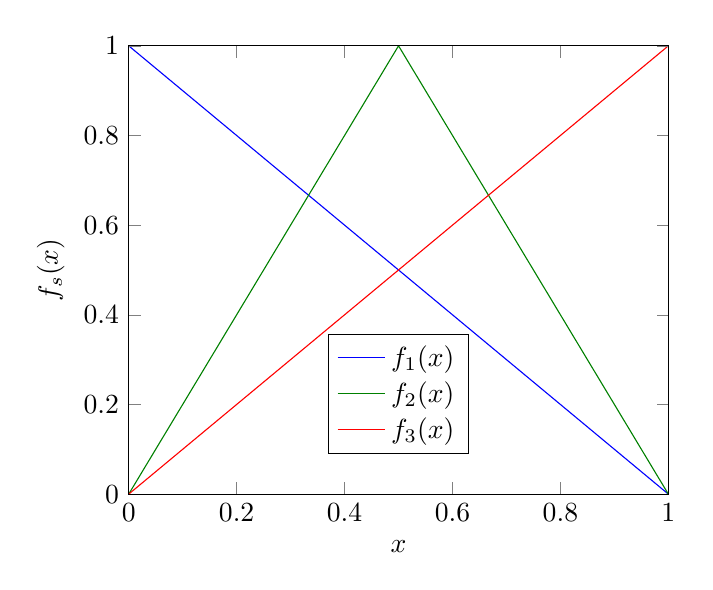
\begin{tikzpicture}
	
	\begin{axis}[
	xlabel={$x$},
	ylabel={$f_s(x)$},
	xmin=0, xmax=1,
	ymin=0, ymax=1,
	axis on top,
	legend style={at={(0.5,0.09)}, anchor=south},
	legend entries={{$f_1(x)$},{$f_2(x)$},{$f_3(x)$}},
	legend cell align={left}
	]
	\addplot [blue]
	table {%
		0 1
		0.5 0.5
		1 0
	};
	\addplot [green!50.0!black]
	table {%
		0 0
		0.5 1
		1 0
	};
	\addplot [red]
	table {%
		0 0
		0.5 0.5
		1 1
	};
	\end{axis}
	
	\end{tikzpicture}
	\caption{Operation of the Centre-Point Triangular Whitenization used in \gls{mtfm}}
	\label{fig:whitenization}
\end{figure}

In the case of the terrestrial communications network used in \cite{Guo11}, the observed metric set $X = {x_1,\dots,x_M}$ representing the measurements taken by each node of its neighbours at least interval, is defined as $X=[$packet loss rate, signal strength, data rate, delay, throughput$]$.

\citet{Guo11} demonstrated that when compared against \gls{otmf} and Hermes trust assessment, \gls{mtfm} provided increased variation in trust assessment over time, providing more information about the nodes' behaviours than packet delivery probability alone can.

\section{Conclusion}
In this chapter, \gls{manet} implementations, topologies, and applications have been explored. 
Further, the concept of a ``Trusting'' network has been explored, both on a abstract theoretical basis, and in the context of a wider development and operational pipeline involving autonomous actors, including a review of current \acrfullpl{tmf}.
These \glspl{tmf} have several aspects that are dependant on assumptions of sufficient available resources and connectivity, that they may not behave as efficiently as would be hoped in constrained or delayful networks, particularly in cases where metric assessment data may be extremely sparse or noisy.

While many aspects of this Trust have been discussed, we are primarily concerned with this problem of assessment of trust through experiential observation of node behaviours in a practical runtime environment, namely the underwater acoustic environment.
In the next chapter, the marine communications environment will be studied, as will the current state of the art in the use of autonomy in defence related maritime applications, and briefly discussing the context of those operations.
%%%%%%%%%%%%%%%%%%%%%%%%%%%%%%%%%%%%%%%%%%%%%%%%%%%%%%%%%%%%%%%%%%%%%%%%%%%%%%%
